% Kota Miura (miura@embl.de)
% Course Textbook: Image Processing and Analysis Basics
% Copyright 2006 - 2011, Kota Miura
%
% This file was converted to LaTeX by Writer2LaTeX ver. 1.0.2
% see http://writer2latex.sourceforge.net for more info
%\documentclass[a4paper]{article}
\documentclass[11pt,a4paper,oneside]{report}
\usepackage{mathpazo} % math & rm
\linespread{1.05}        % Palatino needs more leading (space between lines)
\usepackage[scaled]{helvet} % ss
\usepackage{courier} % tt

%\usepackage[latin1]{inputenc}
\usepackage[T1]{fontenc}
\usepackage[ngerman,english,french,spanish,english]{babel}
\normalfont
\usepackage[footnotesize]{caption}
\usepackage{subfig}
\usepackage{float}

\linespread{1.05}         % Palatino needs more leading (space between lines)
\usepackage{hyperref}
%\hypersetup{colorlinks=true, linkcolor=blue}
\hypersetup{pdftex, colorlinks=true, linkcolor=blue, citecolor=blue, filecolor=blue, urlcolor=blue, pdftitle=CMCI Image processing / Analysis Course Series , pdfauthor=Kota Miura, pdfsubject=, pdfkeywords=}

\usepackage{amsmath}
\usepackage{amssymb,amsfonts,textcomp}
%\usepackage{mathtools}
\usepackage{color}
\definecolor{gray09}{rgb}{0.9,0.9,0.9}  %background for codes
\definecolor{red}{rgb}{1,0,0}
\definecolor{blue}{rgb}{0,0,1}

\usepackage{array}
\usepackage{supertabular}
\usepackage{hhline}
\usepackage[pdftex]{graphicx}

%new commands
\newcommand\textsubscript[1]{\ensuremath{{}_{\text{#1}}}}
\newcommand{\HRule}{\rule{\linewidth}{0.5mm}}

%for header
\usepackage{fancyhdr}
\setlength{\headheight}{15.2pt}
%\pagestyle{fancy}
\pagestyle{fancyplain}
\renewcommand{\chaptermark}[1]{\markboth{#1}{}}
\renewcommand{\sectionmark}[1]{\markright{\thesection\ #1}{}}
 
\lhead{\fancyplain{}{\textit{EMBL CMCI ImageJ Basic Course}}}
\chead{}
\rhead{\fancyplain{}{\textit{\rightmark}}}
\lfoot{}
\cfoot{\fancyplain{}{\thepage}}
\rfoot{}

% space between paragraphs
\parskip 7.2pt

% indent
\setlength{\parindent}{0in} % avoids indent at the beginning of paragraph

\newenvironment{indentexercise}[1]%
{{\setlength{\leftmargin}{2em}}%
\textbf{Exercise \thesubsection-#1}%
\begin{list}{}% 
	\item%
}
{\end{list}}

%indenting for case with Fiji
\newenvironment{indentFiji}%
{\begin{list}{}%
         {\setlength{\leftmargin}{1em}}%
         \item[]%
}
{\end{list}}

%indenting for case with Command Definition
\newenvironment{indentCom}%
{\begin{list}{}%
         {\setlength{\leftmargin}{1em}}%
         \item[]%
}
{\end{list}}

%command for menu tree
\newcommand{\ijmenu}[1]{\texttt{\small#1}}

%command for inline code
\newcommand{\ilcom}[1]{\texttt{\small#1}}

%quick command for making space
 \newcommand{\tab}{\hspace*{3em}}
 
%making 1.5 spaced lines
\usepackage{setspace}
\onehalfspacing

%for inserting PDF 
\usepackage{pdfpages}

%for placing code

% packge for codes
% --- source code matters ---
\usepackage{listings}
%\usepackage{listingsutf8}
\lstset{ %
%language=Octave,                % choose the language of the code
%basicstyle=\footnotesize,       % the size of the fonts that are used for the code
basicstyle=\small\ttfamily, % same as above, but use typewriter
numbers=left,                   % where to put the line-numbers
numberstyle=\footnotesize,      % the size of the fonts that are used for the line-numbers
stepnumber=1,                   % the step between two line-numbers. If it's 1 each line 
                                % will be numbered
numbersep=5pt,                  % how far the line-numbers are from the code
backgroundcolor=\color{gray09},  % choose the background color. You must add \usepackage{color}
keywordstyle=\color{blue}, 	%added
showspaces=false,               % show spaces adding particular underscores
showstringspaces=false,         % underline spaces within strings
showtabs=false,                 % show tabs within strings adding particular underscores
%frame=single,                   % adds a frame around the code
%frame=trBL,
tabsize=2,                      % sets default tabsize to 2 spaces
captionpos=b,                   % sets the caption-position to bottom
breaklines=true,                % sets automatic line breaking
%breakatwhitespace=false,        % sets if automatic breaks should only happen at whitespace
title=\lstname,                 % show the filename of files included with \lstinputlisting;
                                % also try caption instead of title
escapeinside={\%*}{*)},         % if you want to add a comment within your code
morekeywords={*,...},            % if you want to add more keywords to the set
morecomment=[l]{//},
morecomment=[s]{/*}{*/},
morestring=[b]",
%aboveskip={7.2pt}	%supposed to be the space above llisting but dows not work. 
%belowskip={7.2pt}
}

%using eps
\usepackage{epstopdf}

%using natbib
\usepackage{natbib}
\bibpunct{(}{)}{;}{a}{,}{,}
\renewcommand\bibname{References}

% title page matters
% http://sunsite.bilkent.edu.tr/pub/tex/ctan/info/latex-samples/titlepages.pdf
\newcommand*{\titleTH}{\begingroup% T&H Typography
\raggedleft
\HRule\\
\vspace*{\baselineskip}
{\Large Kota Miura}\\[0.167\textheight]

{\bfseries EMBL-CMCI course I}\\[\baselineskip]
{\textcolor{Medium}{\Huge Basics of Image Processing and Analysis}}\\[\baselineskip]
{\small ver 2.1.1}\par
\vfill
%{\Large Centre for Molecular \& Cellular Imaging\\EMBL Heidelberg\\\plogo}\par
{\Large Centre for Molecular \& Cellular Imaging\\EMBL Heidelberg}\par
%
\includegraphics[width=0.15\textwidth]{eps/rgb_logo_2006_win.eps} 

\includegraphics[width=0.07\textwidth]{./Icon30pedge.jpg}\\[1cm] 
\vspace*{3\baselineskip}
\HRule\\
\endgroup}

\definecolor{Dark}{gray}{.2}
\definecolor{Medium}{gray}{.6}
\definecolor{Light}{gray}{.8}

\usepackage{pdfsync}
%%%%%%%%%%%%%%%%%%%%%%%%%%%%%%%%%%%%%%%%%%%%%%%%%%%%%%%%

\begin{document}

\title{Image Processing and Analysis Course I\\
Basics}
\author{Kota Miura\\
\\
  Centre for Molecular and Cellular Imaging,\\
  EMBL Heidelberg,\\
  Germany\\
\\
\texttt{miura@embl.de}
}

\date{\today}

%\maketitle
\pagestyle{empty}
\titleTH
\clearpage
\pagestyle{fancyplain}
\begin{abstract}
\HRule

\textbf{Aim: students acquire basic knowledge and techniques for handling
digital image data by interactively using ImageJ.} \\
\\

NOTE: this textbook was written using the Fiji distribution of ImageJ (IJ ver 1.47n, JRE 1.6.0\_45).
Exercises are recommended to be done using Fiji since most of plugins used in
exercises are pre-installed in Fiji.

Many texts, images and exercises especially for chapter 1.3 and 1.4 were
converted from the textbook of Matlab Image Processing Course in MBL, Woods Hall
(which are originally from a book \textit{Digital Image Processing
using Matlab}, Gonzalez et al, Prentice Hall). I thank Ivan Yudushkin for
providing me with the manual he used there.
Deconvolution tutorial was written by Alessandra Griffa and appears in this
textbook with her kind acceptance to do so.
Figures on stack editing are drawn by S\'{e}bastien Toshi and Julien Colombelli for their course and appear in this textbook for his kind offer. I am pretty much thankful to his figure and am impressed with the way he summarized all the commands related to this.
S\'{e}bastien Toshi also reviewed the article in detail and made may suggestions to improve the text. I thank him a lot for his effort. 


This text is progressively edited. Please ask me when you want to distribute. \\
\\
Compiled on: \today \\
Copyright 2006 - 2014, Kota Miura (http://cmci.embl.de)

\HRule
\end{abstract}
%\setcounter{tocdepth}{3}
%\renewcommand\contentsname{}
%\tableofcontents

\begingroup
\hypersetup{linkcolor=black}
\tableofcontents
\endgroup
\setcounter{chapter}{1}

% section 1
% section 1
% Kota Miura (miura@embl.de)

\section{Basics of Basics}

Handling of digital images in scientific research requires knowledge on
the characteristics of digital image. Signals we see in images are
quantitative information. We are taking pictures, but we are also
measuring signal by numbers. In this section, we learn the very basics
of the numerical nature of digital images. Inappropriate handling not
only lowers the quality of your analysis, but it could also be possible
that your processing is considered as the "manipulation
of data". For this latter point, please also refer to
\citet{Rossner2004}. There are some limits on image processing
to maintain the scientific validity. Standards on scientific image
processing could be found in "Digital Imaging:
Ethics" by \citet{cromey2007}. 

\subsection{Digital image is a matrix of numbers}
\label{subsec:imageEQmatrix}
Digital image we see on computer screen is made up of pixels. We can see
individual pixel by zooming up the image using magnifying tool\footnote{\
Zooming in / out of the image does not change the content of the image.}. Width
and height of the image are defined by the number of pixels in x and y
directions. Each pixel has brightness, or intensity (or more strictly,
amplitude) somewhere between black and white represented as a number. Within
image file saved in computer hard disk, intensity values of pixels are
written. The value is converted to the grayness of that pixel on monitor screen.
We usually do not see these values, or numbers, in the image displayed on
monitor, but we could access these numbers in the image file by converting 
the image file to a text file \footnote{It's also possible in a limited way by
putting mouse pointer over the image and checking the number indicated in
ImageJ menu bar.}.

\begin{indentexercise}{1}
\label{exer:1111}
\item Conversion of image to a text file
\item Make a new image by \ijmenu{[File > New > Image\ldots]}. In dialog window,
make a new image with the following parameters:

\begin{itemize}
\item name = test.txt
\item type = 8bit
\item Fill with Black
\item 10 pixel width
\item 15 pixel height
\item Slices = 1
\end{itemize}


%figure
\begin{figure}[htbp]
\begin{center}
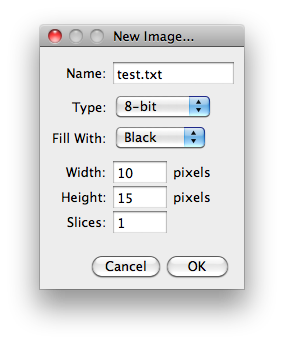
\includegraphics[width=5cm]{img/CMCIBasicCourse201102-img1.png}
\caption{ New Image Dialog}
\label{fig:img1}
\end{center}
\end{figure}
Clicking "OK", you will see a new window showing a black image (Fig.
\ref{fig:mostbasic}). At the top of the window you could see the file dimension ("10 x 15"), 
bit-depth and the file size (I explain these values later.
). Take the pen tool and draw some shape (what ever you want. 
If you do not see anything drawn, then you need to change the color of the pen to white by 
\ijmenu{[Edit > Option > Colors\ldots]} and set Foreground Color to white). 
Then do \ijmenu{[File > Save as > Text image]} and save the file. \\

You will find that the name of the file ends with ".txt". 
Open File Explorer (Win) or Finder (Mac) and double click the file. 
The file will be opened in text editor.

What you see now in the text editor is a "text image", a 2D
matrix of tab-delimited numbers. At the left most column in the example
(Fig. \ref{fig:mostbasic2}), there are only zeros. This corresponds to the left column
pixels in the image, where the color is black. In the middle in the
example image, there are several "255".
These are the white part of the image.
In the text image, edit one of the numbers (either 0 or 255) and change
to 100. Then save the file with a different name, such as
"temp.txt". Then in ImageJ open the file by \ijmenu{[File > Import > Text
Image\dots]}. You should see some difference in the image now. 
The image now has a dark gray dot, not black nor white.
\end{indentexercise}

%double figure
\begin{figure}[htbp]
\centering
\subfloat[]{\label{fig:img2}

\includegraphics[width=3cm]{img/CMCIBasicCourse201102-img2.jpg}
}
\subfloat[]{\label{fig:img3}
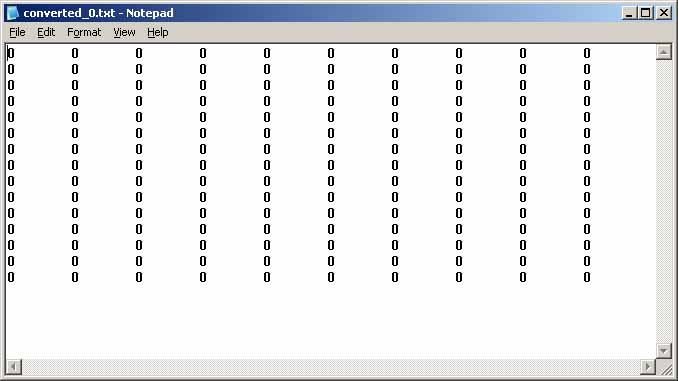
\includegraphics[width=9cm]{img/CMCIBasicCourse201102-img3.jpg}
}
\caption{ A digital image (b) is a matrix of numbers (b).}
\label{fig:mostbasic}
\end{figure} 

%double figure
\begin{figure}[htbp]
\centering
\subfloat[]{\label{fig:img4}
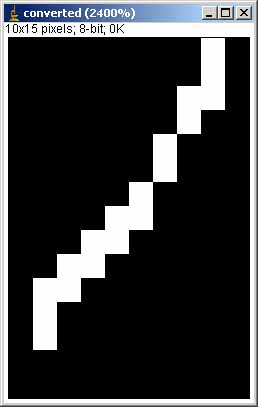
\includegraphics[width=3cm]{img/CMCIBasicCourse201102-img4.jpg}
}
\subfloat[]{\label{fig:img5}
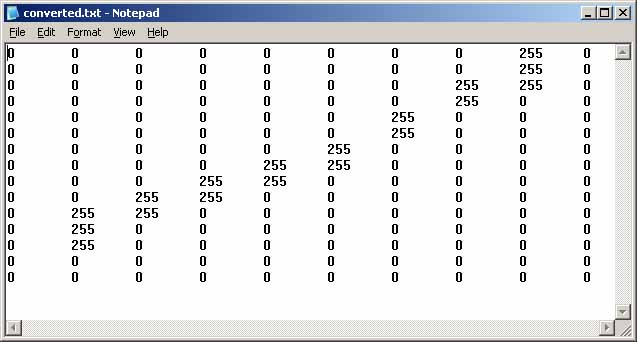
\includegraphics[width=9cm]{img/CMCIBasicCourse201102-img5.jpg}
}
\caption{ White line (a) corresponds to non-zero numbers (b).}
\label{fig:mostbasic2}
\end{figure} 


Note: In hard disk, pixel values are not written as a 2D matrix but as
a single array. Matrix is reproduced after loading according to the width
and height of the image. Pixel values of image stacks (3D or 4D), are
also in 1D array in hard disk. 3D or 4D matrix is reproduced according
to additional information such as slice and channel number. Such
information is written in the
"header" region of the file, which
precedes the "data" region of the
file where the 1D array of pixel array is contained. Header structure
is various depending on the file format, such as TIFF or BMP (we will
see more in "file formats and
header" section). 



\subsection{Image Bit-Depth}

Image file has a defined bit depth. You might have already
heard terms like "8-bit" or
"16-bit" and these are the bit depth. 8-bit
means that the gray-scale of the image has $2^{8} = 256$
steps: in other words, the grayness between black and white is divided
into 256 steps. 16-bit means $2^{16} = 65536$ steps. The
difference is that with 16-bit, one can assign gray-level much more
precise for each pixel; in other words "grayness
resolution" is higher. Microscope images are generated
mostly by CCD camera (or something similar, with matrix of
photo-sensor). CCD chip is a matrix of sensors. Each sensor receives
photons and converts the number received to the grayness number for a
pixel at the corresponding position within the image. Larger bit-depth
enables larger dynamic range with more precise conversion results.~ For
this reason, larger bit-depth is normally recommended for quantitative
imaging. Draw back is that it takes longer time for data transferring
as the bit-depth becomes larger. This may intern limits the time
resolution of image sequences. \\
~\\
Why do we use "$2^{n}$"? This
is because computer uses binary numbers. Minimum units are then 0 or 1.
8-bit means for example a number to be represented as 8-digits binary
number, something like "$00001010$" ( $= 10$ in
decimal). Then the minimum value is =
"$00000000$" ("0" in decimal) and the maximum is $11111111$
("255" in decimal). 8-bit image allows 256
scales for the grayness (using calculator application in your computer,
you could easily convert binary number into normal decimals and vice
versa). In case of 16-bit image, the scale is $2^{16}$ so
there are 65536 steps. 



We must keep in our mind that the nature is continuous. In conventional
mathematics you learn in school, decimal point enables you to represent
infinite steps between 0 and 1. But digitization of the nature loses
the infinite steps such that 0.44 will be rounded to 0 and 0.56 will be
1. Thus, the bit-depth limits the resolution of the analogue to digital
conversion (AD conversion). Higher bit depth generally allows higher
resolution.\\
\\
ImageJ has a high-bit-depth format called signed 32-bit floating point
image. In all above cases with 8-bit and 16-bit, the pixel value is
represented in integer but floating-point type enables decimal points
(real number) for the pixel value such as
"15.445". Though 32-bit floating point
image can be used for image calculation, many functions in ImageJ do
not~work properly so cares should be taken to use this image type. If
you want to know more about the 32-bit format, read the following box
(a bit complicated; you could just pass through)

\begin{quotation}
32 bit FLOATING POINT images utilizes efficient use of the 32 bits.
Instead of using 32 bits to describe 4,294,967,296 integer numbers, 23
bits are allocated to a fraction, 8 bits to an exponent, and 1 bit to a
sign, as follows:\\
~\\
$V = (-1)^{}S * 1.F * 2^{}(E-127)$,\\ 
whereby:\\
S = Sign, uses 1 bit and can have 2 possible values\\
F = Fraction, uses 23 bits and can have 8,388,608 possible
values\\
E = Exponent, uses 8 bits and can have 256 possible values\\
~\\
Practically speaking, this allows for an almost infinite number of tones
between level "0" and
"1", more than 8 million tones between
level "1" and
"2" and 128 tones between level
"65,534" and
"65,535", much more in line with our human
vision than a 32 bit integer image. Because of the infinitesimally
small numbers that can be stored, the 32 bit floating point format
allows to store a virtually unlimited dynamic range. In other words, 32
bit floating point images can store a virtually unlimited dynamic range
in a relatively compact way with more detail in the shadows than in the
highlights and take up only twice the size of 16 bits per channel
images, saving memory and processing power. A higher accuracy format
allows for smoother dynamic and tonal range compression.\\
\\
(Quote from \url{http://www.dpreview.com/learn/?/key=bits})
\end{quotation}




\subsection{Converting the bit-depth of image}

In many occasions, you might want to decrease the bit-depth of image
simply to reduce the file size (16-bit file becomes half the file size
when it is converted to 8-bit), or you might need to use certain
algorithm that is available only with 8-bit images (there are many such
cases), or so on. In any case, this will be a good experience for you
to see the limitation of bit-depth.

Here, we focus on the conversion of a 16-bit image to an 8-bit image to
study its effect and associated possible errors. 


\begin{indentexercise}{1}
Let's first open a 16-bit image from the sample. 
\ijmenu{[File > Open > m51.tif]}. Choose line selection tool and draw a vertical line 
(should be yellow by default: called line ROI). Then do \ijmenu{[Analyze > Plot Profile\ldots]}. 
A window pops up. See figures \ref{fig:img6} and \ref{fig:img7}.

\begin{figure}[htbp]
\begin{center}
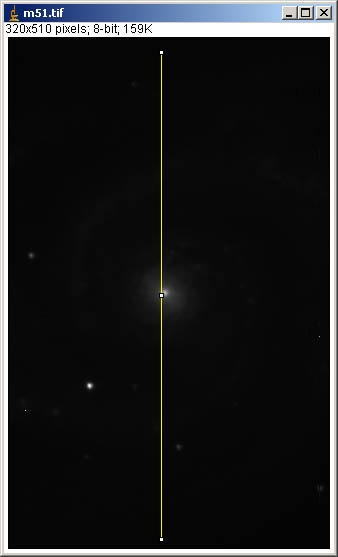
\includegraphics[width=5cm]{img/CMCIBasicCourse201102-img6.jpg}
\caption{Setting a vertical line Roi.}
\label{fig:img6}
\end{center}
\end{figure}

\begin{figure}[htbp]
\begin{center}
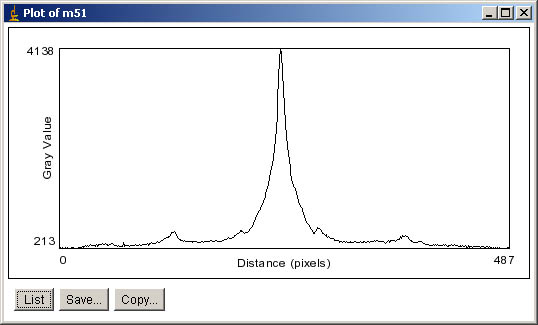
\includegraphics[width=5.694cm,height=3.44cm]{img/CMCIBasicCourse201102-img7.jpg}
\caption{profile of that ROI}
\label{fig:img7}
\end{center}
\end{figure}

Figure \ref{fig:img6} is the profile of the pixel values along the line ROI 
you just have marked on the image (Fig. \ref{fig:img7}). X-axis is the distance 
from the starting point (in pixel) and the y axis is the pixel value along the line ROI. 
The peak corresponds to the bright spot at the center of the image. 

Let's convert the image to 8-bit. First check the state
of "Conversion" option by
\ijmenu{[Edit > Option > Conversion]}. Be
sure that the checkbox "scale when
converting" is off. 

\begin{figure}[htbp]
\begin{center}
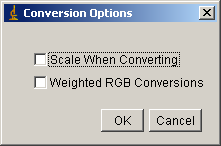
\includegraphics[width=5.847cm,height=3.863cm]{img/CMCIBasicCourse201102-img8.png}
\caption{Conversion Option. Scaling is turned off in this case. }
\label{fig:img8}
\end{center}
\end{figure}


Do \ijmenu{[Image > Type > 8-bit]}. The line
ROI is still there after the conversion. Do \ijmenu{[Analyze > Plot Profile\ldots] }again. 
You will find another graph pops up. Compare the previous profile (16-bit) and the new profile (8-bit).

Conversion causes changes in the y-value. Shapes of the profile look
mostly similar, so if you normalize two images, the curve may overlap.
This is because the image is scaled according to the following
formula.

\[
I_{8}(x,y) = \frac{I_{16}(x, y) - min(I_{16}(x,y))}{ max(I_{16}(x,y)) -  min(I_{16}(x,y))} *255
\]

where

$I_{16}(x, y)$: 16-bit image\\
$min(I_{16}(x,y))$: the minimum value of 16-bit image\\
$max(I_{16}(x,y))$: the maximum value of 16-bit image\\
$I_{8}(x, y)$: 8-bit image\\


Save the line ROI you created by \ijmenu{[Analyze Tools
ROI manager\ldots]}. A small dialog window pops up, so
click "Add" button in the right side.
Number appears in the left side, which indicates the name for the ROI
you made. ROI manager stores coordinates of the start / end points of
the line ROI.

Now, change the option \ijmenu{[Edit > Option >
Conversion]} that the checkbox "scale when
converting" is OFF. Open the 16-bit image again by
\ijmenu{[File > Open > m51.tif]}. Then
again, do \ijmenu{[Image > Type > 8-bit]}.
Apparent difference you see is that now the picture looks like a
overexpose image. Find the ROI manager window and click the ROI number
you stored in above. Same line ROI will appear in the new window. Then
do \ijmenu{[Analyze > Plot Profile\ldots]}. Third profile
shows very different shape compared to previous ones. This is because
the values above 255 is now considered as
"saturated", which means that what ever the
value is, numbers larger than 255 becomes 255.

%figure
\begin{figure}[H]
\begin{center}
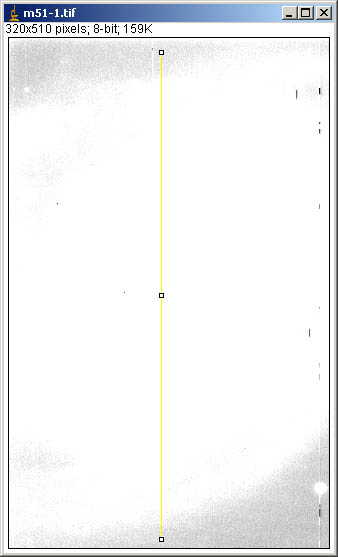
\includegraphics[width=5cm]{img/CMCIBasicCourse201102-img9.jpg}
\caption{ m51 image converted to 8-bit without scaling.}
\label{fig:img9}
\end{center}
\end{figure}

%double figure
\begin{figure}[H]
\centering
\subfloat[]{\label{fig:img10}
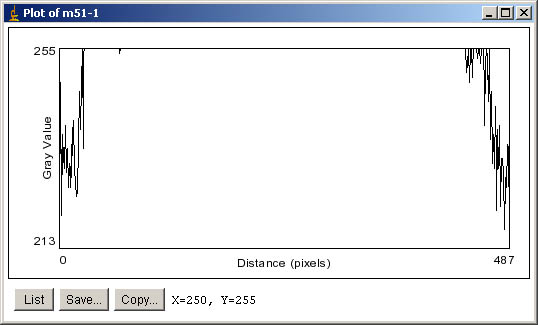
\includegraphics[width=5cm]{img/CMCIBasicCourse201102-img10.jpg}
}
\subfloat[]{\label{fig:img11}
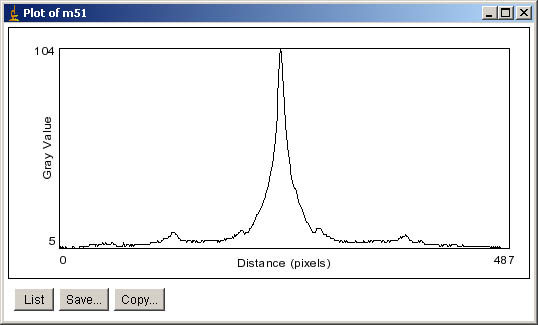
\includegraphics[width=5cm]{img/CMCIBasicCourse201102-img11.jpg}
}
\caption{ (a) Intensity profile of \ref{fig:img5}. If the conversion was done with scaling, then the profile would look like (b). }
\label{fig:8bitConverted}
\end{figure} 

\end{indentexercise}

When you do conversion, very different results could appear depending on
how you scale, like we have just seen. But in many cases, you do not
recognize such changes just by looking at the image: for this reason,
one should keep in mind that the conversion may
"saturate" or cause artifacts in the image
- screwing up scientific images to non-scientific ones. 


\subsection{Math functions}

Digital image is a matrix of numbers. We can calculate images like usual
math. If there is a flat image with pixel value of 10, and if you add 1
to the image, then all pixel values become 11. We think about a pixel
at $(5, 10)$, and we write down the calculation as follows:

\begin{equation}
f(5, 10) = 10
\end{equation}

\begin{equation}
g(5,10) = f (5, 10) +1 = 11
\end{equation}

We generalize this. x and y are the coordinates within the image.

\begin{equation}
g( x , y ) = f (x, y) + 1
\end{equation}

The original image is $f(x, y)$ and the result after the addition
is $g(x, y)$. 

Likewise images could also be subtracted, multiplied and divided by
number. 

\begin{indentexercise}{1}
Simple math on 8-bit image: Prepare a new
image following the initial part of the exercise \ref{exer:1111}. Now,
bring the mouse pointer over the image and check the
"value" that appears in the
status bar in the ImageJ window\footnote{\ In the exercise \ref{exer:1111}, 
we converted the image to a text file and check the pixel
values, but it is also possible to check the value pixel by pixel using
this method.}. All pixel values in the image should be
"value = 0".
"x=\ldots, y=\ldots " in the
status bar. 

Commands for mathematical operations in ImageJ are as follows. 

\ijmenu{[Process > Math > Add\ldots]}\\
\ijmenu{[Process > Math > Subtract\ldots]}\\ 
\ijmenu{[Process > Math > Multiply\ldots]} \\
\ijmenu{[Process > Math > Divide\ldots]}\\

%figure
\begin{figure}[htbp]
\begin{center}
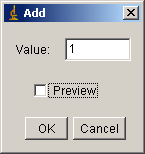
\includegraphics[width=3.8cm]{img/CMCIBasicCourse201102-img12.png}
\caption{ Add dialog.}
\label{fig:img12}
\end{center}
\end{figure}


Add 10 to the image: Do \ijmenu{[Process > Math > Add{\dots]}}. A dialog window pops up so you could
input 10. Press OK button. Now, place the mouse pointer over the image
to check that the pixel values actually became 10. Then select the pen
tool from the tool bar, and draw a diagonal line in the window. Check
again the pixel value. The line you just drew has pixel value 255. Then
add 10 again to the image by \ijmenu{[Process > Math > Add{\dots]}}. Check the pixels by placing the pointer.
The black part is now 20, but what happened to the white line? 

Since the image bit-depth is 8, the available number is only between 0
and 255. When you add 10 to a pixel with its value 255, the calculation
returns 255 because the number
"265" does not exist in 8-bit
world. The similar limitation applies for other calculations also. If
you multiply a pixel value 100 by 3, the answer in normal mathematics
is 300. But in 8-bit world, that pixel becomes 255. 

How about division? Close the currently working test image, and prepare
a new image as you did in \ref{subsec:imageEQmatrix}. Zoom up the image, and add 100
(\ijmenu{[Process > Math > Add{\dots]}}; you
should see the image turns to gray from black). Check pixel values by
placing the pointer above the image. Now, Divide the image by 3
(\ijmenu{[Process > Math > Divide{\dots]}}).
Check the result by placing the mouse over the image. The pixel value
is now 33. Since there is no decimal places in 8-bit, the division
returns the rounded value of (100 / 3 = 33). One could also divide
image by any real number, such as 3.1415. The answer will be in integer
in all cases in 8-bit and 16-bit. In case of floating point 32-bit
image, the calculation results are different. We study this in the next
exercise. 
\end{indentexercise}

\begin{indentexercise}{2}
Simple Math on 32-bit Image: prepare a new
32-bit image (in the \ijmenu{[New > Image..]} dialog,
select 32-bit from the "type"
drop-down menu). Then add 100 to the image. Check that the image pixel
values are all 100. Then divide the image by 3. Check the answer. This
time, answer has decimal places. 
\end{indentexercise}

Bit-depth limitation of digital image is very important for you to know,
in terms of quantitative measurements. Any measurement must be done
knowing the dynamic range of the detection system prior to the
measurement. \textit{If you are trying to measure the amount of
protein, and if some of the pixels are saturated, then your measurement
is invalid}. 

\subsection{Image Math }

In the precious section we calculated using single image. Likewise, we
can do calculation using two images. For example, if there are two
images with a same dimension, and 

\begin{equation}
f(5, 10) = 100
\end{equation}

\begin{equation}
g(5, 10) = 50
\end{equation}

\ldots meaning that the pixel value at the position $(5, 10)$ in the
first image \textit{f} is 100 and in the second image g is 50, we can
add these values and have a third image

\begin{equation}
h(5, 10) = f(5, 10) + g(5, 10) = 100 + 50 = 150
\end{equation}

General form is then as follows that applies to all pixels in the
image:

\begin{equation}
h(x, y) = f(x, y) + g(x, y)
\end{equation}

Note that this only works when the image width and height are
identical. Above is an example of addition. More numerical assignments
are available in ImageJ: \ 

\begin{center}
\tablehead{}
\begin{supertabular}{|m{4.748cm}|m{6.282cm}|}
\hline
\selectlanguage{english}\sffamily Add &
\selectlanguage{english}\sffamily img1 = img1+img2\\\hline
\selectlanguage{english}\sffamily Subtract &
\selectlanguage{english}\sffamily img1 = img1-img2\\\hline
\selectlanguage{english}\sffamily Multiply &
\selectlanguage{english}\sffamily img1 = img1*img2\\\hline
\selectlanguage{english}\sffamily Divide &
\selectlanguage{english}\sffamily img1 = img1/img2\\\hline
\selectlanguage{english}\sffamily AND &
\selectlanguage{english}\sffamily img1= img1 AND img2\\\hline
\selectlanguage{ngerman}\sffamily OR &
\selectlanguage{ngerman}\sffamily img1 = img1 OR img2\\\hline
\selectlanguage{ngerman}\sffamily XOR &
\selectlanguage{ngerman}\sffamily img1 = img1 XOR img2\\\hline
\selectlanguage{ngerman}\sffamily Min &
\selectlanguage{ngerman}\sffamily img1 = min(img1,img2)\\\hline
\selectlanguage{ngerman}\sffamily Max &
\selectlanguage{ngerman}\sffamily img1 = max(img1,img2)\\\hline
\selectlanguage{ngerman}\sffamily Average &
\selectlanguage{ngerman}\sffamily img1 = (img1+img2)/2\\\hline
\selectlanguage{ngerman}\sffamily Difference &
\selectlanguage{ngerman}\sffamily img1 =
{\textbar}img1-img2{\textbar}\\\hline
\selectlanguage{ngerman}\sffamily Copy &
\selectlanguage{ngerman}\sffamily img1 = img2\\\hline
\end{supertabular}
\end{center}


\begin{figure}[htbp]
\begin{center}
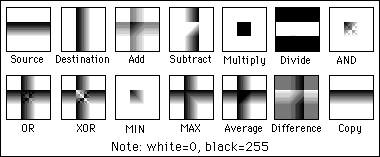
\includegraphics[width=10.945cm,height=4.323cm]{img/CMCIBasicCourse201102-img13.png}
\caption{Taken from ImageJ web site. \url{http://rsb.info.nih.gov/ij/docs/menus/process.html}}
\label{fig:img13}
\end{center}
\end{figure}

\begin{indentexercise}{1}
Image Math -- subtraction:\\
Open Images \textbf{cells\_ActinDNA.tif} and \textbf{cells\_Actin.tif}.
The first image is containing images from two channels. One is actin
labeled, and the other is DNA labeled. We isolate the DNA signal out of
the first image by image subtraction. Do \ijmenu{[Process > Image > Calculator\ldots]}. In the pop-up window, choose the appropriate combination to subtract \textbf{cells\_Actin.tif} from \textbf{cells\_ActinDNA.tif}. Don't forget to turn on the checkbox "Create New Window". 
\end{indentexercise}


\subsection{RGB image}

Color images are in RGB format (could also be so pseudo-color image, or
8-bit color, but this is just because of LUT. See section \ref{subsec:LUT}).
Another popular format is "CMKY" but this
format is optimized for printing purpose (you may have heard it already
when you want to print something in Photolab). RGB stands for three
primary colors. Red, Green and Blue. If all of them are bright at the
same intensity, then the color is white (or gray). If only red is
bright, then the color is red, and so on. A single RGB image thus has
three different channels. In other words, three layers of different
images are overlaid in a single RGB image. Each channel (layer) has a
bit depth of 8-bit. So a single RGB image is 24-bit image. For this,
the file size of color pics becomes three times larger than a grayscale
8-bit image. Don't save 16bit image in RGB format,
since you lose a lot of information, for automatic conversion from 16
to 8 bit takes place. 

\begin{indentexercise}{1}
Working with RGB image:
 
\item (a) Open the image \textbf{RGB\_cell.tif} by \ijmenu{[File > Open]}. Then split the color image to 3 different frames \ijmenu{[Image > Color > Split Channels]}. 

\item (b) Merge three frames by \ijmenu{[Image Color > Merge Channels\ldots]}. 

%figure
\begin{figure}[H]
\begin{center}
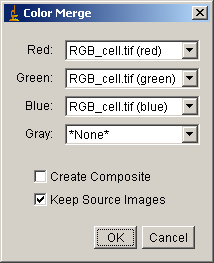
\includegraphics[width=5cm]{img/CMCIBasicCourse201102-img14.png}
\caption{ Color Merge Dialog}
\label{fig:img14}
\end{center}
\end{figure}

In the dialog window, choose an image name for each channel. Uncheck
"Create Composite" and check
"keep source images". Then try
swapping color assignments to see the effect. 

\item (c) Working on each channel separately: Close all windows and
open the "RGB\_cell.tif". Do
\ijmenu{[Image > Color > Channel Tools\ldots]}. Then click button "More" and select "Create Composite".
%figure
\begin{figure}[H]
\begin{center}
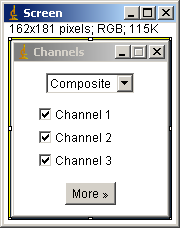
\includegraphics[width=4cm]{img/CMCIBasicCourse201102-img15.png}
\caption{ Channel Tool}
\label{fig:img15}
\end{center}
\end{figure}

Resulting image is a three-layer stack and each layer corresponds to one
of R, G or B. Each layer can be processed individually. 
%figure
\begin{figure}[H]
\begin{center}
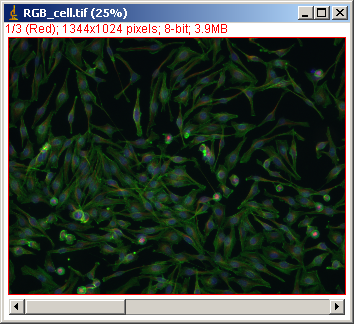
\includegraphics[width=9cm]{img/CMCIBasicCourse201102-img16.png}
\caption{ Composite image. Note slider at the bottom for switching between three channels.}
\label{fig:img16}
\end{center}
\end{figure}

Using Channel Tools again,
%figure
\begin{figure}[H]
\begin{center}
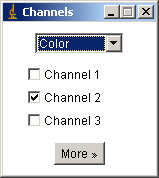
\includegraphics[width=4cm]{img/CMCIBasicCourse201102-img17.png}
\caption{ Channel Tool, now only selected for Channel 2.}
\label{fig:img17}
\end{center}
\end{figure}

Choose "color" from the pull-down tab, instead of "Composite". Select channel 2 (in this image, this will be Green channel). Select a part of the image using Rectangular ROI. 
%figure
\begin{figure}[H]
\begin{center}
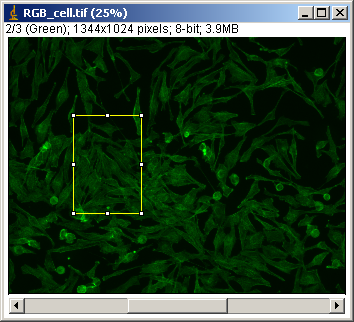
\includegraphics[width=9cm]{img/CMCIBasicCourse201102-img18.png}
\caption{ ROI selection, in channel 2. Note the position of slider.}
\label{fig:img18}
\end{center}
\end{figure}

Then do \ijmenu{[Edit > Clear]}. This will pop up a window. 
%figure
\begin{figure}[H]
\begin{center}
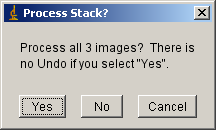
\includegraphics[width=4cm]{img/CMCIBasicCourse201102-img19.png}
\caption{ Asking you whether you want to process all channels.}
\label{fig:img19}
\end{center}
\end{figure}

Click No, because you want to process only one channel. 
%figure
\begin{figure}[H]
\begin{center}
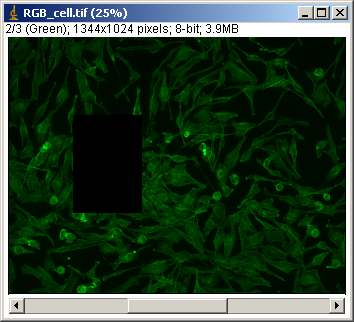
\includegraphics[width=9cm]{img/CMCIBasicCourse201102-img20.png}
\caption{ Channel 2 pixel values inside selected ROI becomes 0.}
\label{fig:img20}
\end{center}
\end{figure}
\begin{quote}
\textit{Troubleshooting}: If the ROI is not cleared (becomes bright), then you should change the background color setting. Do \ijmenu{[Edit > Option > Colors\dots]} and you will see a pop-up window like this. 
%figure
\begin{figure}[H]
\begin{center}
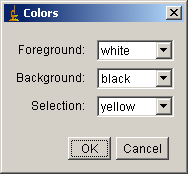
\includegraphics[width=4cm]{img/CMCIBasicCourse201102-img21.png}
\caption{ Color selection dialog.}
\label{fig:img21}
\end{center}
\end{figure}

Make sure that the background is "black". Do the ROI clearing again. 
\end{quote}
Select "Composite" in the pull-down tab of channel tool. 
%figure
\begin{figure}[H]
\begin{center}
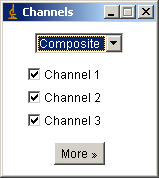
\includegraphics[width=4cm]{img/CMCIBasicCourse201102-img22.png}
\caption{ Choosing Composite, all channels visual.}
\label{fig:img22}
\end{center}
\end{figure}

Resulting image should look like below. 
%figure
\begin{figure}[H]
\begin{center}
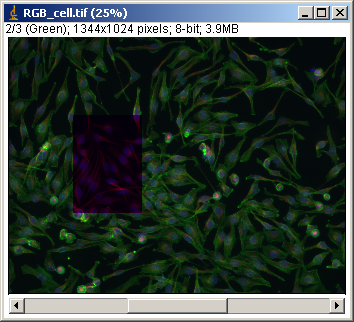
\includegraphics[width=9cm]{img/CMCIBasicCourse201102-img23.png}
\caption{ Only channel2 is devoid of image within the selected ROI.}
\label{fig:img23}
\end{center}
\end{figure}

In this case, green channel intensity in green channel ROI is now set to 0 ("clear"). You could do such
processing of single channel by simply selecting a channel by horizontal scroll bar and do the processing directly, such as drawing square ROI and deleting that part in that channel in "composite" view. 
\end{indentexercise}

\subsection{Look-Up Table }
\label{subsec:LUT}

We now look at how matrix of numbers is converted to actual image. Let"s think about a row of pixels with increasing pixel values from 0 to 255 (so there are 256 pixels in this row). Computer monitor will show a gradient of intensity that is linearly increasing its brightness from black to white. This is because the software is giving a command to the monitor, such that "this pixel $(x, y)$ is 158 so the corresponding voltage required for this position $(x, y)$ in the screen should be **mV". For this command to be composed, software needs a so called "look-up table" (LUT). 


This is just like a situation when you start checking a menu in a
restaurant with limited amount of money in your pocket. Say you want to
eat a pizza. You have only \texteuro 10 in your pocket. Looking at the
pizza menu, you will not try to find what you want from names of pizza
and what are the toppings, but instead you will check the prices listed
in the right side of the menu trying to figure out which pizza is less
then \texteuro 10. When you find \texteuro 7.5 in the list, then you slide your
sight to the left side of the menu, and find out that the pizza is
"Margherita". Similar to this,
software first checks the pixel value and then goes to the look-up
table (menu) to find out which brightness should be passed to the
monitor as a command ( = find a convincing price in the menu, then
sliding your sight to the left and find out which pizza to order).



\begin{indentexercise}{1}
For 8-bit images, there is a default LUT normally called "grayscale". To see the LUT, open the image \textbf{Cell\_Colony.jpg} and then do \ijmenu{[Image > Color > Show LUT]}. LUT window pops up showing the relationship between pixel value and pixel intensity. Try change the LUT by \ijmenu{[Image > Lookup Tables >Spectrum]}. Pixel value does not change by this operation, but the pixel intensity changes that the image appears differently now. Check the LUT again by do \ijmenu{[Image > Color > Show LUT]}. 
\end{indentexercise}

%double figure
\begin{figure}[H]
\centering
\subfloat[]{\label{fig:img24}
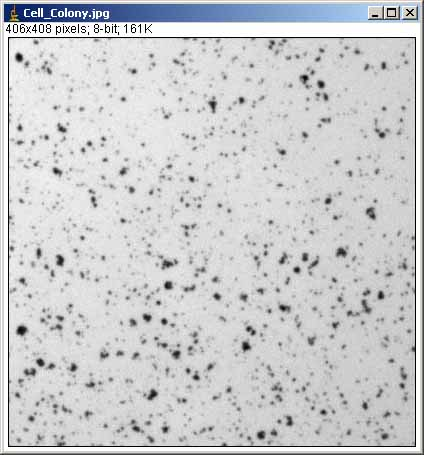
\includegraphics[width=6.371cm,height=6.853cm]{img/CMCIBasicCourse201102-img24.jpg}
}
\subfloat[]{\label{fig:img25}
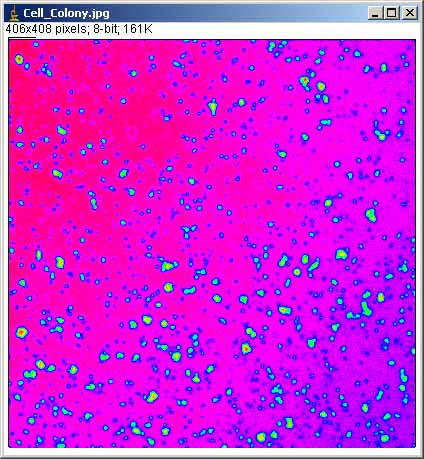
\includegraphics[width=6.431cm,height=6.962cm]{img/CMCIBasicCourse201102-img25.jpg}
}
\caption{ Grayscale LUT (a) converted to spectrum LUT (b).}
\label{fig:LUTconversionImages}
\end{figure} 

%double figure
\begin{figure}[H]
\centering
\subfloat[]{\label{fig:img26}
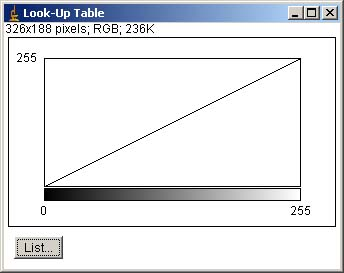
\includegraphics[width=6.055cm,height=4.805cm]{img/CMCIBasicCourse201102-img26.jpg}
}
\subfloat[]{\label{fig:img27}
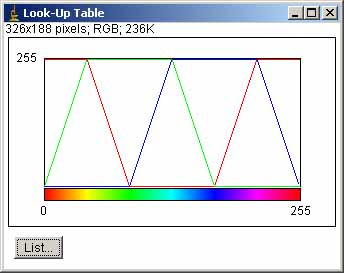
\includegraphics[width=6.103cm,height=4.833cm]{img/CMCIBasicCourse201102-img27.jpg}
}
\caption{ (a) Grayscale LUT and (b) spectrum LUT}
\label{fig:LUT[lots}
\end{figure} 

\subsection{Image File Formats: Header and Data, Stacks, Multi-dimensional images}

Image file contains two types of information. One is the image data, the matrix of numerical values. Another is called "header", which contains the information about the architecture of image. Since software must know information such as bit-depth, width and height, and the size of the header before opening the image, the information is written in the "header". The total file size of an image file is then 

$Total file size = header size + data size$

There are many different types of image formats, such as TIFF, BMP, PICT and so on. Each format has differently sized header, and also the location of the information. In biology, microscope companies create their own formats to include more parameters about the image, such as the type of microscope used, used objectives, binning, shutter speed, time intervals, user name and so on. 

Presence of company-specific formats complicates us because that image could only be openable from software provided by that company. For this reason, there are an excellent Plug-in which enable importing of specific format to ImageJ \footnote{\tab LOCI Bioformat Plugin:\\
\url{http://www.loci.wisc.edu/ome/formats.html}}

You do not have to know all the details about the architecture of various image formats (thanks to the bioformats plugin), but it is important for you to know that the difference resides mainly in the header. The data part is in most cases same, something like what we have seen already using text image (for more details on header, refer to the appendix \ref{app1} ). 

\textit{Multidimensional data}: When you take time-lapse images or z-stack, then there will be a series of images with same prefix and serial number like image0001.tif, image0002.tif, image0003.tif\dots\ and so on. These files could be imported by ImageJ and watch the sequence like a movie. Such an image series is called "stack" in ImageJ and can be saved as a single file. File extension is typically ".tif", which is same as the single frame file. In Metamorph, popular software used in biology, uses .stk as the file extension. These files can be loaded directly in ImageJ. We will study more on the actual use of the image stacks in section \ref{sec:timeseries}.

\textit{Compression}: Another important point that we must keep in our mind is that we should not compress data, if you want to get some numbers out of them. Popular compression formats are like JPEG and GIF. Compression of images deals with throwing away redundant part or mathematically interpolating some parts of the image. This causes artifacts in the image and it could even be "manipulation" of data. We must avoid using compression for the images we use for measurements. These compression formats are also called "lossy" formats, as the process of compression loses data. PNG is a compression format that does not alter the original pixel values.

\begin{indentexercise}{1}
Open the example image \textbf{wt1.tif}. Do
\ijmenu{[Image > Show Info\dots]}. Scale (pixels/inch)
is listed in the information window, which was read out from the header
of the image. Then do \ijmenu{[Image > Properties]},
also showing the scale. 
\end{indentexercise}

\subsection{Resizing images. (Shrinking and Enlarging) }

When we say "resizing" images, this
does not mean zooming in or out the image\footnote{\ Zooming is done by
the magnification tool (icon of magnification glass) and this simply
enlarges or shrinks the pixels, not modifying the original data. \par
}. Resizing changes the original data. If we have an image of size 10
pixels by 10 pixels and resize it to 200\%, the image becomes 20 x 20.
If we resize it by 50\%, then the image becomes 5 x 5. Resizing is a
simple task that could be done by \ijmenu{[Image > Adjust > Size\ldots]}. This is a simple operation but one must
take care about how pixels will be produced while enlarging and reduced
while shrinking. If the enlarging is simply two times larger, we could
imagine that each pixel will be copied three times to produce a block
of four pixels to complete the task. The pixel values of the newly
inserted pixels will then be identical to the source pixel. 

But what happens if we want to enlarge the image by 150 \%? To simplify
the situation, think about an image with 2 x 2 pixels. Then the
resulting image becomes 3 x 3. To understand the effect, do the
following exercise. 


\begin{indentexercise}{1}
Open the example image
4pixelimage\_sample.tif. The image is ultra small, so zoom it
up to the maximum (as much as you can, you must click on or
\textit{Ctrl - +}). You now see four pixels in the window.
Duplicate the image by \ijmenu{[Image > Duplicate]}.
Magnify again. "Select all" by
\ijmenu{[Edit > Selection > Select All]}.
Then \ijmenu{[Image > Adjust > Size\ldots]}.
In the dialog window, input the width 4 and height 4 (corresponds to
200\% enlargement). Turn on the check box "aspect
ratio" on and
"Interpolation" off. Then click
OK. Check the pixel values in original image, and the enlarged image.
\end{indentexercise}

\begin{indentexercise}{2}
Do the similar resizing, but this time enlarge
the image by 150\%. Check the pixel values.
%double figure
\begin{figure}[htbp]
\centering
\subfloat[]{\label{fig:img28}
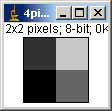
\includegraphics[width=3.951cm,height=3.916cm]{img/CMCIBasicCourse201102-img28.jpg}
}
\subfloat[]{\label{fig:img29}
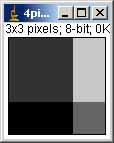
\includegraphics[width=4.022cm,height=5.045cm]{img/CMCIBasicCourse201102-img29.jpg}
}
\caption{ Artifacts produced by resizing. (a) Four pixel image and (b) nine pixel image after
resizing. }
\label{fig:resizing}
\end{figure} 

\end{indentexercise}

The resizing in the exercise was without interpolation -- the check box
was OFF. Interpolation is similar to the one dimensional interpolation
we do with graphs. In case of images, the gradient is also two
dimensional so the situation is a bit more complex. There are various
methods for interpolating image. The interpolation method used in
ImageJ is the \textit{bilinear interpolation}. Briefly, the bilinear
interpolation algorithm samples pixel values in the surrounding of the
insertion point, and calculates the pixel value for that
position\footnote{\ For more details on bilinear interpolation, refer
to\\
http://www.cambridgeincolour.com/tutorials/image-interpolation.htm.}.
One must keep in mind that the result of enlarging or shrinking of
image depends on the interpolation method -- and scientific results
could be altered depending on the method you use.

\clearpage
\subsection{ASSIGNMENTS }%%%%%%%%%%%%%%%%%%%%%%%

\textbf{\sffamily
Assignment 1-1-1: Digital image = matrix of numbers}

Edit a text image using text editor. Be sure to insert space between
numbers as separator. Save the text file and open it as an image in
ImageJ by importing text image function. \ \ 

\textbf{\sffamily
Assignments 1-1-2: bit depth}
\begin{enumerate}
\item How many gray scale steps does a 12-bit image have?\\
\item Describe in text how a 1-bit image looks like.
\end{enumerate}

\textbf{\sffamily
Assignment 1-1-3: bit depth conversion}

Use m51.tif (16-bit!) sample image to draw a plot profile, as we did in
the course. In the profile plot window, a
"list" button is at the left-bottom corner.
Click the button. You will then see a new window containing a column on
numbers. These numbers can be copy \& pasted to spread sheet software
such as Openoffice Calc or MS Excel. Overlay three curves in a graph,
and discuss the difference in two different ways of bit-conversions. 

\textbf{\sffamily
Assignments 1-1-4: Simple math with Image}
\begin{enumerate}
\item Try subtracting certain values from the image you created in
the Assignment 1-1-1 and check that the values cannot be less than 0. 
\item Prepare an 8-bit image with pixel value 200. Divide the
image by 3, and check the answer. 

\item Prepare a 16-bit image. In the \ijmenu{[File > New > 
Image\ldots]} dialog, select 16-bit from the
"type" drop-down menu. Try adding
certain value to check the maximum pixel value. 

\item Discuss why measurement of fluorescence intensity using
digital image is invalid when some pixels are saturated. 
\end{enumerate}

\textbf{\sffamily
Assignments 1-1-5: LUT}

Open "Cell\_Colony.tif". Use LUT edit function and design your own LUT to highlight the black dots in
Green and the background in Black. "LUT editor" can be activated by \ijmenu{[Images > Color > Edit LUT\ldots]}. Instruction for the LUT editor is at\\
\url{http://rsb.info.nih.gov/ij/plugins/lut-editor.html} \\
You might be able to manage using it without reading the web instruction; just try!). LUT (.lut file) could also be edited using Excel. 

\textbf{\sffamily
Assignments 1-1-6: File size and image bit depth, image size}

If there is an image with width = 100 pixels and height = 200 pixels,
what would be the expected size of the image file in bytes? 1 byte =
8-bit.

Create a new image with the dimension as above, and save the image in
"bitmap (.bmp)" format and check the file
size. Is it same as you expected, or different? Save the same image in
text file format and check the file size again.

\textbf{\sffamily
Assignment 1-1-7 Resizing}

\begin{enumerate}
\item Enlarge the sample image 4pixelimage\_sample.tif by
150\% while the "Interpolation"
check box in the size adjustment window is ON. Study the pixel values
before and after the enlargement. What happened? Describe the result.

\item Change "canvas size" by \ijmenu{[Image > Adjust > Canvas Size]} for any image. What"s the
difference to "Resize"?
\end{enumerate}



% section 2
% section 2
% Kota Miura (miura@embl.de)

\section{Intensity}

An image has only one type of information: a distribution of intensity. The image analysis in biology deals with this distribution in quantitative ways. We investigate the distribution from different angles using various algorithms and analyze biological phenomena such as shapes, cell movements and protein-protein interactions. For example in GFP labeled cells, intensity of signal is directly related to the density of the labeled biological component.
We now start studying how to interpret signals, and how to extract biologically meaningful numerical values out of intensity distribution. 

\subsection{Histogram}
\label{subsec:histogram}

If there is an 8-bit image with 100 pixel width and 100pixel height,
there are 10,000 pixels. Each of these pixels has certain pixel value.
Intensity histogram of an image is a plot that shows distribution of pixel counts over a range of pixel values, 
typically its bit depth or between the minimum and the maximum pixel value with in the image. 
Histogram is useful for examining the signal and
background pixel values for determining a threshold value to do segmentation.
We will study image threshold in \ref{sec:segmentation}). 


\begin{indentexercise}{1}
Open \textbf{Cell-Colony.tif}. Do
\ijmenu{[Analyze > Histogram]}. A new window appears. The
x-axis of the graph is pixel value. Since the image bit-depth is 8-bit,
the pixel values ranges from 0 to 255. The y-axis is the number of
pixels (so the unit is [count]). Since 255 = white and 0 = black, the
histogram has long tail towards the lower pixel value. This reflects
the fact that the image has white background and black dots.

Check pixel values in the histogram by placing the mouse pointer over
the plot and move it along the x axis. Pixel count appears at the
bottom of the histogram window. Switch to the cell colony image, and
place the pointer over dark spot. Read the pixel value there, and then
try finding out the number of pixels with the same value in the
histogram. What is the range of pixel values which corresponds to the
spot signal?  
\end{indentexercise} 
Histogram could also be used for enhancing contrast of image. Several
different algorithms are available for this: histogram normalization,
histogram equalization and local histogram normalization. 

If the histogram is occupying only part of the available dynamic range
of image bit depth (8-bit: 0 -- 255, 16-bit: 0 -- 65535), we could
adjust pixel values of image to increase its range so that contrast become more
enhanced. There are two ways to do this: normalization and
equalization. 

\subsubsection{Normalization}

With normalization, pixel values are normalized according to the
minimum and the maximum pixel values in the image and bit-depth. If the minimum pixel value is
\textit{pmin} and the maximum is \textit{pmax} in an 8-bit image, then normalization is done as follows:

\begin{equation*}
\mathit{NewPixelValue}=\frac{(\mathit{OriginalPixelValue}-\mathit{pmin})}{(\mathit{pmax}-\mathit{pmin})}\ast
255
\end{equation*}

\subsubsection{Equalization}

Equalization converts pixel values so that the values are distributed
evenly within the dynamic range. Instead of describing this in detail
using math formula, I will explain it with a simple example (see Fig. \ref{fig:equalizationSimple}). 
We consider an image with its pixel value ranging
between 0 and 9. We plot the histogram from this image, the result looks
like in the figure \ref{fig:img30}. For equalization, a cumulative
plot is first prepared from such histogram. This cumulative plot is computed by progressively integrating the histogram values (see 
Fig. \ref{fig:img31}, black curve).
To equalize (flatten) the pixel intensity distribution within the range 0-9, we would ideally require a straight diagonal
cumulative plot (in other words, the probability density of the 
pixel intensity distribution should be near-flat). To get such plot, we need to compensate the histogram by shifting values from the bars 5 and 7 to the bars 7 and 9, respectively (now, bars are in
red after shifting). After this shifting the cumulative plot now looks
more straight and diagonal (Fig. \ref{fig:img31} right, red curve).


%double figure
\begin{figure}[H]
 \centering
 \subfloat[]{\label{fig:img30}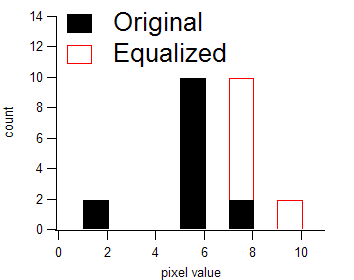
\includegraphics[height = 45mm]{fig/CMCIBasicCourse201102-img30.png}}
 \subfloat[]{\label{fig:img31}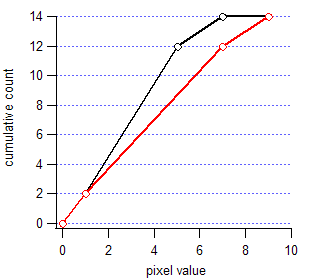
\includegraphics[height = 45mm]{fig/CMCIBasicCourse201102-img31.png}}
 \caption{ (a) Histogram Equalization: Very simple case.
The actual calculation uses cumulative plots (b) of the histogram of original
image, and uses it as a look up table to convert original pixel value,
applied point-by-point. }
 \label{fig:equalizationSimple}
\end{figure}

\begin{indentexercise}{2}
Histogram Normalization and Equalization:
\item Open sample image \textbf{g1.tif}, and then duplicate the image by
\ijmenu{[Image > Duplicate]}. Click the duplicate and then \ijmenu{[Image > Process > Enhance Contrast]}. A dialog window pops up. Set "Saturated Pixels" to 0.0\% and check "Normalize", while unchecking "Equalize Histogram", then click OK.
Compare histogram of original and normalized images .  

\item Duplicate g1.tif again by \ijmenu{[Image > Duplicate]}. Click the
duplicate and then \ijmenu{[Image > Process > Enhance Contrast]}. A dialog window pops up. Set "Saturated
Pixels" to 0.0\% and uncheck "Normalize", while check "Equalize Histogram", then click OK.
Compare histogram of original, normalized and equalized images
(\ijmenu{[Analyze > Histogram]}).

\end{indentexercise}

\begin{indentexercise}{3}
Local Histogram Equalization (Optional):
\item Histogram equalization could also be performed on a local basis. This becomes
powerful, as more local details could be contrast enhanced. You could
try this with the same image g1.tif, by \ijmenu{[Pligins > CMCICourseModules > CLAHE]} 
(if you have installed the course plugin in ImageJ) or if you are using Fiji, \ijmenu{[Process > Enhance Local Contrast (CLAHE)] }
\end{indentexercise}



\subsection{Region of Interest (ROI) }
\label{subsec:roi}
To apply certain operation to a specific part of the image, you can
select a region by "region of interest
(ROI)" tools. The shape of the ROI could be various,
such as rectangular, elliptical, polygon, free hand or a line
(straight, segmented or free hand). There are several functions that
will be used often in association with ROI tools. 

\begin{indentexercise}{1}
Cropping. Open any image. Select a region by
rectangular ROI. Then \ijmenu{[image > Crop]}. This will
remove the unnecessary part of the image, to reduce calculation time.
\end{indentexercise}

\begin{indentexercise}{2}
Masking. Open any image. Select a region by
rectangular ROI. Then \ijmenu{[Edit > clear]}.
\ijmenu{[Edit > Clear Outside]}. After checking what
happened, do \ijmenu{[Edit Fill]}. (same operation could
be done by \ijmenu{[Edit > Selection > Crate Mask]})
\end{indentexercise}

\begin{indentexercise}{3}
Invert ROI. Open any image. Select a region by
rectangular ROI. Then\ijmenu{ [Edit > Selection > Make Inverse]}. In this way, you can select region
excluding the region you initially selected.
\end{indentexercise}

\begin{indentexercise}{4}
Redirecting ROI. Open any two images. In one
of the image, select a region by rectangular ROI. Then activate the
other image by clicking that window, and do \ijmenu{[Edit > Selection > Restore Selection]}. ROI with
same size and position will be reproduced in the window. 
\end{indentexercise}



\begin{indentexercise}{5}
ROI manager. You can store the position and
size of the ROI in the memory. Select a region by rectangular ROI.
\ Then \ijmenu{[Analysis > Tools > Roi Manager]}. Click "Add" button to store
ROI information. Stored ROI can be saved as a file, and could be loaded
again when you restart the ImageJ.
\end{indentexercise}


\subsection{Intensity Measurement}

As you move the mouse pointer over individual pixels, their intensity value are indicated in the ImageJ menu bar. This is the easiest way to
read pixel intensities, but you can only get the values one by one. Here we learn a way to get statistical information of a group
of pixels within ROI. This has more practical usages for research. 

To measure pixel values of a ROI, ImageJ has a function \ijmenu{[Analyze >
Measure]}. Before using this function, you could specify the parameters 
you want to measure by \ijmenu{[Analyze > Set measurements]}. There are many parameters
in the "Set measurement" window. Details on these parameters are listed in the
Appendix \ref{app2}. For intensity measurements following parameters are
important.


\begin{itemize}
\item \textbf{Mean Gray Value} - Average gray value within the selection. This
is the sum of the gray values of all the pixels in the selection
divided by the number of pixels. Reported in calibrated units (e.g.,
optical density) if Analyze/Calibrate was used to calibrate the image.
For RGB images, the mean is calculated by converting each pixel to
grayscale using the formula $gray=0.299red+0.587green+0.114blue$ or the
formula $gray=(red+green+blue)/3$ if "Unweighted RGB to
Grayscale Conversion" is checked in Edit/Options/Conversions.

\item\textbf{Standard Deviation}{}- Standard deviation of the gray values.

\item\textbf{Min \& Max Gray Level} - Minimum and maximum gray values within
the selection.

\item\textbf{Integrated Density} - The sum of the values of the pixels in the
image or selection. This is equivalent to the product of Area and Mean
Gray Value. The Dot Blot Analysis example demonstrates how to use this
measurement to analyze a dot blot assay.
\end{itemize}

A short note on image-based fluorometry: In biochemical experiments,
scientists measure protein concentration by measuring absorbance of UV
light or by labeling proteins with dyes or fluorescence and measure the
intensity of emission. This is because light absorbance or the
intensity of fluorescence intensity is proportional to the density of
protein in the irradiated volume within cuvette. Very similar to this
when fluorescence image of cells are taken, pixel values (which is the
fluorescence intensity) are proportional to the density of the labeled
protein at each pixel positions. For this reason, measurement of
fluorescence intensity using digital imaging could be considered as the
two dimensional version of the conventional fluorometry. 

\begin{indentexercise}{1}
\item Open a sample image \textbf{cells\_Actin.tif}. Before actually executing the measurement,
do \ijmenu{[Analyze > Set Measurements]}. A dialog
window opens. There are many parameters listed in the upper-half of the
window.

%figure
\begin{figure}[htbp]
\begin{center}
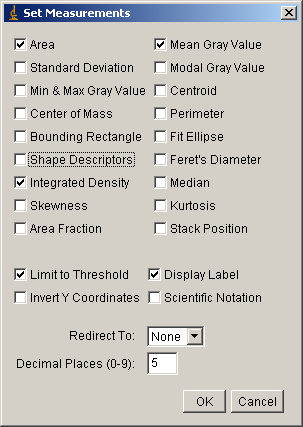
\includegraphics[width=8.017cm,height=11.298cm]{fig/CMCIBasicCourse201102-img32.png}
\caption{Set Measurement Window}
\label{fig:img32}
\end{center}
\end{figure}


The parameters we select now are:
\begin{itemize}
\item Area
\item Integrated Density 
\item Mean Gray Value
\end{itemize}

Check the box of these three parameters. Integrated density is the sum
of all the pixel values and Mean Gray Value is the average of all the
pixel values within ROI. So 

$Integrated Density = Area * Mean Gray Value$

Select one of the cells in cell\_Actin.tif image and zoom it up
using magnifying tool. Switch the tool to
"Polygon" tool. Draw polygon ROI around
the cell. Then do \ijmenu{[Analyze > Measure]}. A window
titled "Results" pops-up, listing the
measured values. Check that the integrated density is the
multiplication of area and the mean gray value.




%double figure
\begin{figure}[htbp]
 \centering
 \subfloat[]{\label{fig:img33}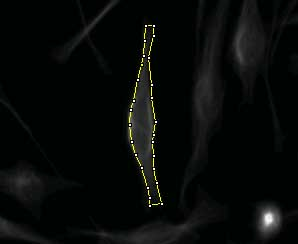
\includegraphics[height=4cm]{fig/CMCIBasicCourse201102-img33.jpg}}
 \subfloat[]{\label{fig:img34}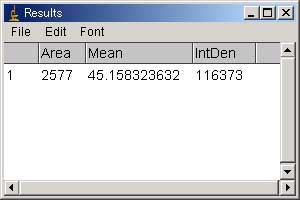
\includegraphics[height=4cm]{fig/CMCIBasicCourse201102-img34.jpg}}
 \caption{ (a) Tracing Cell Edge by Segmented ROI and Measuring the Intensity within selected area. }
 \label{fig:CellIntensityMeasurement}
\end{figure} 

This value is not the actual intensity of the fluorescence within the
cell since it also includes the background intensity (offset).
Measure the background intensity by creating a new ROI in the area
where there is no cell.

%figure
\begin{figure}[htbp]
\begin{center}
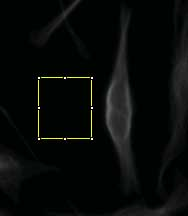
\includegraphics[height=4.5cm]{fig/CMCIBasicCourse201102-img35.jpg}
\caption{Measurement of Background}
\label{fig:img35}
\end{center}
\end{figure}

\end{indentexercise}

NOTE: When no ROI is active (no yellow bounding rectangle or so),
then the measurement is performed on the whole image.

\subsection{Image transformation: Enhancing Contrast}
\label{subsec:enhancecontrast}
Some of you might already have experience with the contrast enhancing of
digital images, since in most of imaging software like the ones that
come with digital camera usually have this function. Low contrast images
have small difference in the tones and the objects are difficult to observe.
If the contrast is too high, then the tone difference is so much that
the picture is "over exposed".
Adjustment of contrast controls the tone difference to optimize the
visual resolution. The contrast enhancement primarily changes the LUT,
so that the original image data is unaffected (you will see in the
following exercise). The original data is changed only when you click
"Apply" button. Then the pixel values
are re-scaled according to the LUT you set.



Care must be taken for contrast enhancement since pixel values are
altered. This could be regarded as
"fraud" or
"manipulation" in science, especially if
you are measuring image intensity. If all images that you are trying to
compare were equally contrast enhanced,
then the images could eventually be compared. Even then, there will be another
pit-fall if you artificially saturate the image: this happens often
especially in the case of low bit-depth images. 

\begin{indentexercise}{1}
Open image gel\_inv.tif. Do \ijmenu{[Image > Adjust > Brightness/Contrast]}. 
Pop-up window appears which looks like the
figure below (left). The graph shown in the upper part of the window is 
the
histogram of the image just like you have seen in section \ref{subsec:histogram} Histogram. 
Since the image is 8-bit, scale in the x axis is 0 to 255.
There is also a black diagonal line. This corresponds to the LUT of the
image on the screen: pixel values in x is translated into the gray
value on the screen (brightness on the screen is y-axis). 

The slope and position of the LUT can be altered by click and dragging
four sliding bars under the graph, each with the name minimum, maximum,
brightness and contrast. Try changing these values and studying the
effect on the image. 

QUESTION: What is the problem with the adjustment shown in the
right side of the figure below?

%double figure
\begin{figure}[htbp]
 \centering
 \subfloat[]{\label{fig:img36}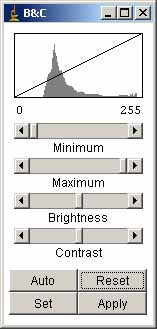
\includegraphics[width=2.762cm,height=5.803cm]{fig/CMCIBasicCourse201102-img36.jpg}}
 \subfloat[]{\label{fig:img37}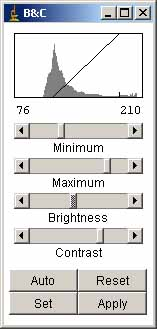
\includegraphics[width=2.762cm,height=5.803cm]{fig/CMCIBasicCourse201102-img37.jpg}}
 \caption{ (a) Histogram of \textbf{gel\_inv.tif} before enhancing contrast. (b) Some bad adjustments example. }
 \label{fig:quizEnhanceContrast}
\end{figure} 

\end{indentexercise}

\begin{indentexercise}{2}
Continued from above: the original image file
is not changed at this stage. When you push
"Apply" button at the bottom-right
corner, the original image is altered numerically. Try set the LUT as
you like, and push the Apply: what happened to the Histogram and the
LUT indicator? (you can always
"Undo" the "Apply" by \ijmenu{[Edit > Undo]}, 
or revert to the original file by \ijmenu{[File > Revert]}).
\end{indentexercise}

\begin{indentexercise}{3}
With RGB image, it is possible to adjust the
brightness and contrast for individual color channel. Open the image
\textbf{RGB\_cell.tif}, then do \ijmenu{[Image > Adjust > Color Balance]}. 
There is a pull-down menu to specify
the channel you want to change. Try changing different channels to
optimize the image. 
\end{indentexercise}

\subsection{Image correlation between two images: co-localization plot}

In many experiments we need to compare the
localization of two or more proteins and examine whether those proteins
are co-localized. In many cases this has been evaluated by visual
inspections. But with digital images, it is possible to evaluate the
degree of co-localization more quantitatively. This is done by plotting
a so called "co-localization
plot". To do this in ImageJ one could download a
plugin \textbf{Colocalization\_Finder}\footnote{download from \url{http://rsb.info.nih.gov/ij/plugins/colocalization-finder.html}}
and install it.

The level of colocalization could be then parametrized by using statistical
values such as Pearson's coefficient and
Mander's coefficient. These values have advantages and
disadvantages depending on the image properties. For detailed
description on these issues, refer to \citet*{BolteJM2006}.

Additional insights, pitfalls and tips on localizing spot signals could
be found in \citet{Waters2009}. This paper also provides detailed examination of the precision of dot detections. 
\clearpage

\subsection{ASSIGNMENTS}

\textbf{\sffamily
Assignment 1-2-1:}

Suppose that you have an 8-bit grayscale image showing three objects of 
distinct intensities against a bright background. What would
the corresponding histogram look like?

\textbf{\sffamily
Assignment 1-2-2: }

With image \textbf{cell\_Actin.tif}, do the measurement with 4 cells and one background in image as we did in the
exercise. This time, store ROI in ROI manager (refer to \ref{subsec:roi} Roi)
and do the measurement at once. First, you store 5 different ROI one by
one ("Add" button). Then click "Show all" button in the ROI manager.
Activate all ROI by clicking the ROI name in the list while pushing
down the SHIFT key. Then click "Measure"
button. All five ROI will be measured at once. Average the values and
describe the results in text.

\textbf{\sffamily
Assignment 1-2-3: }
\begin{enumerate}
\item Optimize the contrast of image
\textbf{m51\_8bit.tif}. Be careful not to
saturate the pixels so you don't throw away important
information in the lower pixel values. Check the histogram.
Don't close the histogram window

\item After applying the adjustment above (clicking
"Apply" button), check the histogram
again. Compare the histogram before and after. What happened? Discuss
the reason.
\end{enumerate}

% section 3
% section 3
% Kota Miura (miura@embl.de)

\section{Filtering}

Filtering improves the appearance of digital image. Then recognition of
shapes becomes easier by noise removing and enhancement of the
structural edge. Not only for the appearance, filtering improve the
efficiency of "segmentation" which we
will study in the next section. Segmented image could be used as a mask
to specify regions to be measured. Note that the filtering alters the
image so one must realize that in most cases, processed images cannot
be used for quantitative intensity measurement without precise
knowledge on what would happen to the numerical values after the
processing. 

There are two different types of filtering: one involves the frequency
domain of images (Fourier transformed image), while the others deals
with spatial domain. We first study the spatial domain filtering and
its central concept "convolution", and
walk through various types of convolutions. We then study the frequency
domain filtering (FFT). In FFT world, convolution of an image with
filter kernel could be done simply by multiplication between two
images. 



\subsection{Convolution}\label{subsecConvolution}

In the \ijmenu{[Process]} menu, we see a long list of
filters. An important concept for understanding what these commands
will do to your image is "convolution".
A small mask (called kernel) is moved along the image pixel by pixel
and apply operations using the surrounding pixel values (see Fig.
\ref{fig:img38}). The result of operation is over-written to that pixel position
as the new pixel value.


%figure
\begin{figure}[htbp]
\begin{center}
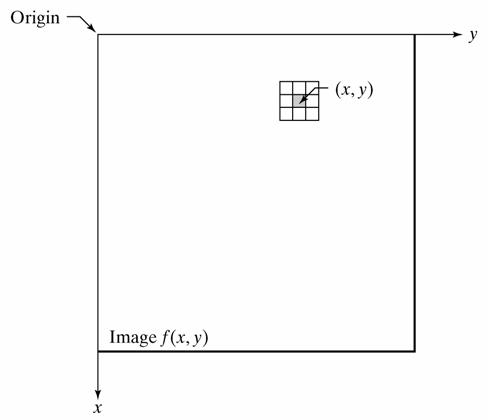
\includegraphics[width=7cm]{img/CMCIBasicCourse201102-img38.png}
\caption{ An image and a Kernel (figure taken from DIP)}
\label{fig:img38}
\end{center}
\end{figure}


To understand how the convolution is done, we take a one-dimensional
example (Fig. \ref{fig:img39}).


%figure
\begin{figure}[htbp]
\begin{center}
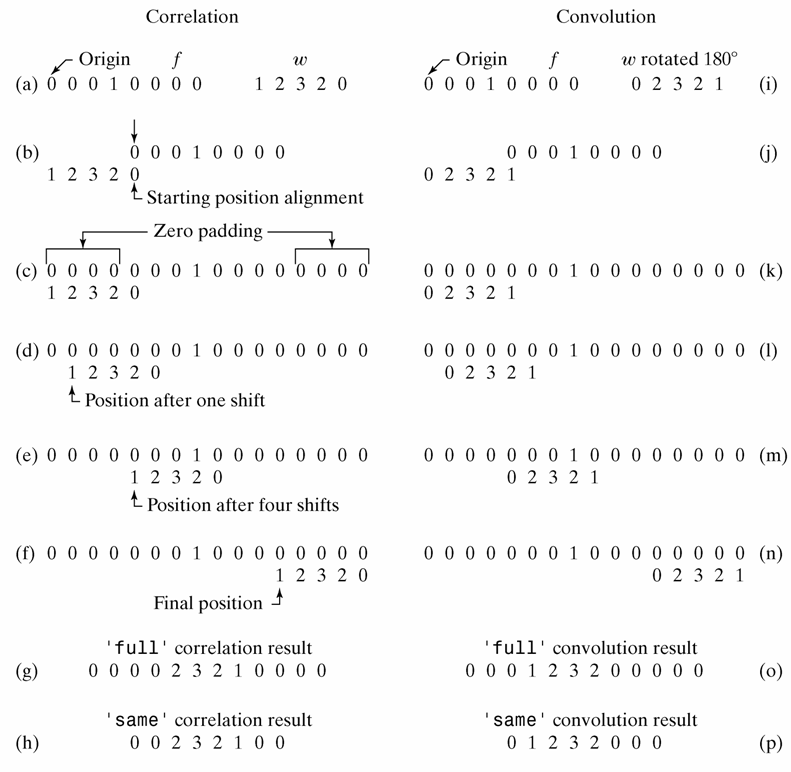
\includegraphics[width=11.718cm]{img/CMCIBasicCourse201102-img39.png}
\caption{ 1-dimensional convolution and correlation (figure taken from DIP)}
\label{fig:img39}
\end{center}
\end{figure}

We have a small 1D array $f$, and we want to convolve a
kernel $w$ (i). We first rotate the kernel by 180 degrees that
the order is now reversed. Then we align $f$ and $w$ to
match the position of the last element of kernel to the first element
of $f$. Since we want to have all the kernel elements to have
corresponding partner, we "pad" $f$ by 0.
This is just for the convenience of calculation (k). Then you multiply
each element pairs (5 pairs in this case) and sum up the results. since
all partners in $f$ are 0, the sum of multiplication is 0. We note this
as the first element of "full convolution
result" (o). We then slide $w$ to the left by one
element, do the multiplications and summing up again. Note the result
as the second element of "full convolution
result" (o). Like wise, we do such calculation step by
step until last element of $w$ matches the last element of
$f$ (n). After then, we throw away padded elements from the
output 1D array to have a resulting array with same length as the
original $f$ (p). 

%{\selectlanguage{english}\sffamily

\begin{quote}
{\sffamily\bfseries
Convolution and correlation}

Two closely-related bilinear operations that are especially important
for information processing are $convolution$ and
$correlation$. In the simplest case, correlation can
be described as a comparison of two fields at all possible relative
positions. More specifically, if $\chi$
is the correlation of two one-dimensional fields $\phi$
and $\psi$, $\chi = \phi*\psi$, then $\chi(r)$ reflects how well 
$\phi$ and $\psi$ match (in an inner-product sense) when relatively displaced by
$r$. Mathematically, 
\[
\chi(r)=\int_{\Omega }^{} \phi(s-r)\psi (s)ds
\]
Higher dimensional correlations are the same, except that $r$ is
a relative displacement $vector$ rather than a scalar. 

$Convolution$, $\chi=\phi\otimes \psi$, is essentially the same as correlation, except that the field $\phi$ is reflected before the comparison takes place: 
\[
\chi(r)=\int_{\Omega }^{}  \phi(r-s)\psi  (s)ds
\]
Convolution is useful because: (1) its algebraic properties are more
like multiplication, and thus more familiar, than correlation; and (2)
many physical processes (e.g. linear systems, such as dendritic nets)
perform convolutions.

%Two closely-related bilinear operations that are especially important
%for information processing are \textit{convolution} and
%\textit{correlation}. In the simplest case, correlation can
%be described as a comparison of two fields at all possible relative
%positions. More specifically, if 
%
\includegraphics[width=0.185cm,height=0.344cm]{img/CMCIBasicCourse201102-img40.png}
%is the correlation of two one-dimensional fields 
%
\includegraphics[width=0.212cm,height=0.503cm]{img/CMCIBasicCourse201102-img41.png}
%and 
%
\includegraphics[width=0.212cm,height=0.503cm]{img/CMCIBasicCourse201102-img42.png}
%, 
%
\includegraphics[width=1.455cm,height=0.503cm]{img/CMCIBasicCourse201102-img43.png}
%, then 
%
\includegraphics[width=0.635cm,height=0.556cm]{img/CMCIBasicCourse201102-img44.png}
%reflects how well 
%
\includegraphics[width=0.212cm,height=0.503cm]{img/CMCIBasicCourse201102-img45.png}
%and 
%
\includegraphics[width=0.212cm,height=0.503cm]{img/CMCIBasicCourse201102-img46.png}
%match (in an inner-product sense) when relatively displaced by
%\textit{r}.\href{http://www.cs.utk.edu/~mclennan/anon-ftp/FCMC-tr/footnode.html#516}{
%
\includegraphics[width=0.397cm,height=0.397cm]{img/CMCIBasicCourse201102-img47.png}
%}
% Mathematically, 
%
%
\includegraphics[width=13.227cm,height=0.716cm]{img/CMCIBasicCourse201102-img48.png}
%
%Higher dimensional correlations are the same, except that \textit{r} is
%a relative displacement \textit{vector} rather than a
%scalar. 
%
%\textit{Convolution}, 
%\includegraphics[width=1.561cm,height=0.503cm]{img/CMCIBasicCourse201102-img49.png}
%, is essentially the same as correlation, except that the field 
%\includegraphics[width=0.212cm,height=0.503cm]{img/CMCIBasicCourse201102-img50.png}
%is reflected before the comparison takes place: 
%
%\includegraphics[width=13.227cm,height=0.716cm]{img/CMCIBasicCourse201102-img51.png}
%
%Convolution is useful because: (1) its algebraic properties are more
%like multiplication, and thus more familiar, than correlation; and (2)
%many physical processes (e.g. linear systems, such as dendritic nets)
%perform convolutions.


Quote from:
\url{http://www.cs.utk.edu/\~mclennan/anon-ftp/FCMC-tr/node14.html}
\end{quote} 

In two dimensional matrix, see the example in Fig. \ref{fig:img52}. 

%figure
\begin{figure}[htbp]
\begin{center}
\includegraphics[width=10cm]{img/CMCIBasicCourse201102-img52.png}
\caption{ Two-dimensional convolution (figure taken from DIP)}
\label{fig:img52}
\end{center}
\end{figure}

The matrix (a) is first padded (b), then starting from the top-left
corner (f) the matrix is convoluted (g) and then the padded rows and
columns are removed to return an output matrix with the same dimension
as the original (h).

\subsection{Kernels}

In \ijmenu{[Process]} menu, we have many operators such
as smooth, sharpen, find edges\dots and so on. Many of them ate
called "linear filters" because
the result of filtering is a linear combination of the original image
pixel values. We study various kernels in this section. 

\subsubsection{Smoothening}
\ "Smoothening" operation, which is
used for attenuating noise (Median kernel is better for shot-noise
removal but for learning purpose we stick to the smoothing), is done by
applying the following kernel to the image. 

%\includegraphics[width=1.305cm,height=1.87cm]{img/CMCIBasicCourse201102-img53.png}
\[
 \begin{matrix}
  1 & 1 & 1 \\
  1 & 1 & 1 \\
  1 & 1 & 1
 \end{matrix}
\]

Let"s take an example of an image with a vertical line
in the middle.


\[
 \begin{matrix}
  0 & 0 & 10 & 0 & 0 \\
  0 & 0 & 10 & 0 & 0 \\
  0 & 0 & 10 & 0 & 0 \\
  0 & 0 & 10 & 0 & 0 \\
  0 & 0 & 10 & 0 & 0 
 \end{matrix}
\]

%\includegraphics[width=2.928cm,height=3.104cm]{img/CMCIBasicCourse201102-img54.png}

Just for now, we forget about the padding for explanation, and first
apply the kernel to the top-left corner for
calculating convolved value at (1, 1) pixel position (note: top-left element position is (0, 0)).
Then the calculation is


$output( 1 , 1 )$\\
$\quad = ( 0 \times 1 + 0 \times 1 + 0 \times 1 + $\\
$\qquad 0 \times 1 + 0 \times 1 + 0 \times 1 + $\\
$\qquad 10 \times 1 + 10 \times 1 + 10 \times 1 ) / 9 $\\
$\quad = 30 / 9 $\\
$\quad = 3$

The sum of multiplication is divided by 9, which is the sum of all
elements in the kernel. This is to normalize the convolution, so that
the output value will not to be too large compared to the original. We
then shift the kernel one step in x-direction, and apply the kernel for
calculating (2, 1) position. 

$output( 2 , 1)$\\
$\quad = ( 0 \times 1 + 0 \times 1 + 0 \times 1 + $\\
$\qquad 10 \times 1 + 10 \times 1+ 10 \times 1 +$\\ 
$\qquad 0 \times 1 + 0 \times 1 + 0 \times 1) / 9 $\\
$\quad = 30 / 9$\\ 
$\quad = 3$

You might have now understood that the
"smooth" operation is actually
averaging the values in the surrounding. Applying the kernel through
the image, the new image will be: 

%\includegraphics[width=2.752cm,height=3.104cm]{img/CMCIBasicCourse201102-img55.png}

\[
 \begin{matrix}
  0 & 2 & 2 & 2 & 0 \\
  0 & 3 & 3 & 3 & 0 \\
  0 & 3 & 3 & 3 & 0 \\
  0 & 3 & 3 & 3 & 0 \\
  0 & 2 & 2 & 2 & 0 
 \end{matrix}
\]
The vertical line is then now broader and darker -- the smoothing
effect. Note that the pixels in the first and the 5th rows were
calculated with zero padding so that values are 2 rather than 3. This
is the boundary effect unavoidable with any filtering by convolution.
We could attenuate this effect if we do padding by duplicating
neighboring pixels. Then the result of convolution then becomes

%\includegraphics[width=2.681cm,height=3.104cm]{img/CMCIBasicCourse201102-img56.png}
\[
 \begin{matrix}
  0 & 3 & 3 & 3 & 0 \\
  0 & 3 & 3 & 3 & 0 \\
  0 & 3 & 3 & 3 & 0 \\
  0 & 3 & 3 & 3 & 0 \\
  0 & 3 & 3 & 3 & 0 
 \end{matrix}
\]

\begin{indentexercise}{1}
 Working with kernel: in ImageJ, one could
design original kernel and do convolution for images.
Open \textbf{microtubule.tif} image and
zoom up so you can see individual pixels. Do \ijmenu{[Process
> Filter > Convolve]}. A pop-up window
appears (see the image below). One could edit the kernel. Be sure to
make spaces between numbers. By clicking OK, the kernel will be applied
to the image. 

Try replacing the default kernel with the smoothening kernel we studied
above. Apply the kernel to sample image
\textbf{microtubule.tif}. Increase the
dimension to 5 x 5, 9 x 9 and do the smoothening. 

\textbf{Question}: what happened when the size of the kernel became
larger? Check the preview option, so that the change in the kernel
could be visualized directly while editing.

%figure
\begin{figure}[htbp]
\begin{center}
\includegraphics[width=4.471cm]{img/CMCIBasicCourse201102-img57.png}
\caption{ Convolver Window.}
\label{fig:img57}
\end{center}
\end{figure} 

\end{indentexercise}

\subsubsection{Sharpen }

%\includegraphics[width=2.258cm,height=1.87cm]{img/CMCIBasicCourse201102-img58.png}
\[
 \begin{matrix}
  -1 & -1 & -1 \\
  -1 & 12 & -1 \\
  -1 & -1 & -1
 \end{matrix}
\]

This kernel sharpens the image, also known as Laplacian. Side effect:
noise is also enhanced. 


\subsubsection{Find Edge (gradient)}
\label{subsub:findedgekernel}
Following two kernels are applied independently. Square root of the sum
of the square of two result images will be calculated (called
"Sobel Filter": for more details,
see Appendix \ref{app3}) \ 

%\includegraphics[width=2.364cm,height=1.87cm]{img/CMCIBasicCourse201102-img59.png}
\[
 \begin{matrix}
  1 & 2 & 1 \\
  0 & 0 & 0 \\
  -1 & -2 & -1
 \end{matrix}
\]
and

%\includegraphics[width=1.87cm,height=1.87cm]{img/CMCIBasicCourse201102-img60.png}
\[
 \begin{matrix}
  1 & 0 & -1 \\
  2 & 0 & -2 \\
  1 & 0 & -1
 \end{matrix}
\]


\subsubsection{Gaussian Blur}

This kernel blurs (in positive sense, we call it
"smooth") the image by convolution
using a square Gaussian (bell-shaped) kernel. The width of the kernel,
in pixels, is 2*\textit{sigma}+1, where \textit{sigma} is entered into
a dialog box (ImageJ documentation). Following three kernels are with
different sigma 2 (5x5), 3 (7x7) and 7 (15x15). 

Gauss 5 x 5 (Sigma = 2)
 
%\includegraphics[width=2.785cm,height=3.104cm]{img/CMCIBasicCourse201102-img61.png}
\[
 \begin{matrix}
  1 & 1 & 2 & 1 & 1\\
  1 & 2 & 4 & 2 & 1\\
  2 & 4 & 8 & 4 & 2\\
  1 & 2 & 4 & 2 & 1\\
  1 & 1 & 2 & 1 & 1
 \end{matrix}
\]

Gauss 7 x 7 (Sigma = 3)

%\includegraphics[width=4.163cm,height=4.374cm]{img/CMCIBasicCourse201102-img62.png}
\[
 \begin{matrix}
  1 & 1 & 1 & 2 & 1 & 1 & 1\\
  1 & 2 & 2 & 4 & 2 & 2 & 1\\
  2 & 2 & 4 & 8 & 4 & 2 & 2\\
  2 & 4 & 8 & 16 & 8 & 4 & 2\\
  2 & 2 & 4 & 8 & 4 & 2 & 2\\
  1 & 2 & 2 & 4 & 2 & 2 & 1\\
  1 & 1 & 1 & 2 & 1 & 1 & 1
 \end{matrix}
\]
Gauss 15 x 15 (Sigma = 7)

%\includegraphics[width=10.76cm,height=9.454cm]{img/CMCIBasicCourse201102-img63.png}
% to make a large matrix, http://newsgroups.derkeiler.com/Archive/Comp/comp.text.tex/2008-07/msg00905.html
\setcounter{MaxMatrixCols}{16}
\[
\begin{matrix}
  2 & 2 & 3 & 4 & 5 & 5 & 6 & 6 & 6 & 5 & 5 & 4 & 3 & 2 & 2\\
  2 & 3 & 4 & 5 & 7 & 7 & 8 & 8 & 8 & 7 & 7 & 5 & 4 & 3 & 2\\
  3 & 4 & 6 & 7 & 9 & 10 & 10 & 11 & 10 & 10 & 9 & 7 & 6 & 4 & 3\\
  4 & 5 & 7 & 9 & 10 & 12 & 13 & 13 & 13 & 12 & 10 & 9 & 7 & 5 & 4\\
  5 & 7 & 9 & 11 & 13 & 14 & 15 & 16 & 15 & 14 & 13 & 11 & 9 & 7 & 5\\
  5 & 7 & 10 & 12 & 14 & 16 & 17 & 18 & 17 & 16 & 14 & 12 & 10 & 7 & 5\\
  6 & 8 & 10 & 13 & 15 & 17 & 19 & 19 & 19 & 17 & 15 & 13 & 10 & 8 & 6\\
  6 & 8 & 11 & 13 & 16 & 18 & 19 & 20 & 19 & 18 & 16 & 13 & 11 & 8 & 6\\
  6 & 8 & 10 & 13 & 15 & 17 & 19 & 19 & 19 & 17 & 15 & 13 & 10 & 8 & 6\\
  5 & 7 & 10 & 12 & 14 & 16 & 17 & 18 & 17 & 16 & 14 & 12 & 10 & 7 & 5\\
  5 & 7 & 9 & 11 & 13 & 14 & 15 & 16 & 15 & 14 & 13 & 11 & 9 & 7 & 5\\
  4 & 5 & 7 & 9 & 10 & 12 & 13 & 13 & 13 & 12 & 10 & 9 & 7 & 5 & 4\\
  3 & 4 & 6 & 7 & 9 & 10 & 10 & 11 & 10 & 10 & 9 & 7 & 6 & 4 & 3\\
  2 & 3 & 4 & 5 & 7 & 7 & 8 & 8 & 8 & 7 & 7 & 5 & 4 & 3 & 2\\
  2 & 2 & 3 & 4 & 5 & 5 & 6 & 6 & 6 & 5 & 5 & 4 & 3 & 2 & 2
 \end{matrix}
\]
\setcounter{MaxMatrixCols}{10}

\subsubsection{Median}
None-linear filters are so called because the result of applying the
filter is non-linear. Median filter used for the removal of noise is
one of such filters. In ImageJ, the command will be \ijmenu{[Process >
Filter > Median]}. Following is the
principle of how median filter works. When we apply median filter with
a 3 x 3 size, ImageJ samples 3 x 3 neighbors surrounding the target
pixel. Graphically, if the sampled region looks like below (target
position contains 2 now) 

%\includegraphics[width=1.552cm,height=1.87cm]{img/CMCIBasicCourse201102-img64.png}
\[
 \begin{matrix}
  1 & 7 & 9 \\
  4 & 2 & 8 \\
  6 & 5 & 3
 \end{matrix}
\]

Then we align these numbers in the ascending order. 

\ \ 1 2 3 4 5 6 7 8 9

We take the median of this sequence ($=5$) and replace the value 2 with
5.
\subsection{Morphological Image Processing}

Mathematical morphology is a powerful tool that can be used to extract
features and components from an image. It is often used to pre-process
or post-process of images to facilitate analysis. In this process a
small shape (structuring element, not necessarily square like we did in
the precious section) is translated across the image during the course
of processing. Certain mathematical logic operations are performed on
the image using the structuring element to generate the processed
image.
In this section, we first introduce dilation and erosion, two
fundamental operations in mathematical morphology. We then describe
morphological operations obtained by combining erosion and dilation. 
\subsubsection{Dilation}
Dilation is an operation that grows objects in a binary image. The
thickening is controlled by a small structuring element. In Fig. \ref{fig:img65} 
you can see the structuring element on the right and
the result after applying dilation on a rectangle.

 \begin{figure}[htbp]
 \begin{center}
 \includegraphics[width=9.222cm]{img/CMCIBasicCourse201102-img65.png}
 \caption{ Dilation (figure taken from DIP).}
 \label{fig:img65}
 \end{center}
 \end{figure}



\subsubsection{Erosion}
Erosion shrinks or thins objects in a binary image. After erosion the
only pixels that survive are those where the structuring element fits
entirely in the foreground (Fig. \ref{fig:img66}).

%figure
\begin{figure}[htbp]
\begin{center}
\includegraphics[width=8cm]{img/CMCIBasicCourse201102-img66.png}
\caption{ Erosion (figure taken from DIP)}
\label{fig:img66}
\end{center}
\end{figure}

In above examples structuring elements are asymmetrically shaped. In
ImageJ, structuring elements are squares so the dilation: erosion
effects are even along both axes. 

\begin{indentexercise}{1}
Load noisy-fingerprint.tif and broken-text.tif. Apply dilations or
erosions with different iterations. 

For setting iterations, do \ijmenu{[Process > Binary > Options]}. 
Binary option window opens and you can set
several parameters. "Count"
matters with setting the number of overlapping pixels between
structuring element and the object that determines output 0 or 1.
Larger count causes less degree of erosion or dilation.

%figure
\begin{figure}[htbp]
\begin{center}
\includegraphics[width=4cm]{img/CMCIBasicCourse201102-img67.png}
\caption{ Setting Iteration.}
\label{fig:img67}
\end{center}
\end{figure}
\end{indentexercise}

\begin{quote}
From ImageJ manual: Iterations specifies the number of times erosion,
dilation, opening, and closing are performed. Count specifies the
number of adjacent background pixels necessary before a pixel is
removed from the edge of an object during erosion and the number of
adjacent foreground pixels necessary before a pixel is added to the
edge of an object during dilation. Check Black Background if the image
has white objects on a black background.
\end{quote}

\subsection{Morphological processing: Opening and Closing}

Combinations of morphological operations can be very useful in removing
many artifacts present in images. This will become very useful after
segmenting an image. The first operation we will see is opening, which
is an erosion followed by dilation. Opening smooths object contours,
breaks thin connections and removes thin protrusions. After opening,
all objects smaller than the structuring element will disappear.
Closing is a dilation followed by erosion. Closing smooths object
contours, joins narrow breaks, fills long thin gulfs and fills holes
smaller than the structuring element.

\begin{indentexercise}{1}
Load noisy-fingerprint.tif and broken-text.tif. Apply
opening and closing to the images by \ijmenu{[Process 
> Binary > Open]} and \ijmenu{[Process > Binary > Close]}. 
\end{indentexercise}


\begin{indentexercise}{2}
(Optional) Next, we do morphological processing using anisotropic structuring
element. 

Invoke \ijmenu{[Plugins > CMCICourseModules > Morphology]} and design vertical structuring element first with (1)
diameter = 3. This is simply by inputting
"3" in the Diameter field. Click tiles
to activate/deactivate positions. Click
"Apply" button to do the actual
processing. Then you could try with a larger diameter: (2) diameter =
9. Apply these two different structuring elements to dilate
noisy-finger print. Discuss the difference in outputs. 


%figure
\begin{figure}[htbp]
\begin{center}
\includegraphics[width=6.5cm]{img/CMCIBasicCourse201102-img68.png}
\caption{ Morphological Image Processing dialog, to design structuring element.}
\label{fig:img68}
\end{center}
\end{figure}
\end{indentexercise}

\subsection{Minimum and Maximum}

Morphological transformation on grayscale image is very useful for
subtracting the background, such as to eliminating the shading of the
image such as shown in fig below. Opening and closing we studied above
works only with binary images. For gray scale images, one can use
Minimum (like Open) and Maximum (like Close) under [Process
Filters]. One could remove all features smaller than
the structuring element by "Minimum"
operation of gray images. In the following example we will experience
this.

\begin{indentexercise}{1}
\label{exer:removerice}
Open rice.tif. Then \ijmenu{[Process > Filters > Minimum]}. In the dialog
window, input the radius of the structuring element (structuring
element is circular). Find a radius that removes rice from the image.
Successfully removed image is the background image. Then remove the
background image from the original image. 

\textit{Note}: For bright field images, background actually should
be removed by division rather than subtraction such as: 
\[
Corrected\_Image = \frac{Specimen - Darkfield}{Brightfield - Darkfield} * 255
\]
\end{indentexercise}



\subsection{Background Subtraction}

Besides the background subtraction we studied above using Minimum and
Maximum filtering, there are special function designed for the
background subtraction (extension of morphological processing). ImageJ
has a direct background subtraction by Rolling ball algorithm \footnote{
Stanley Sternberg's article, "Biomedical Image Processing", IEEE Computer, January 1983). }
In the dialog window when you execute this operation, you will be asked for
the Rolling ball radius. This should be at least as large as
the radius of the largest object in the image that is not part of the
background.

%figure
\begin{figure}[htbp]
\begin{center}
\includegraphics[width=11.875cm]{img/CMCIBasicCourse201102-img69.jpg}
\caption{ Background Subtraction (from ImageJ site).}
\label{fig:img69}
\end{center}
\end{figure}


\begin{indentexercise}{1}
Open rice.tif. Do background
subtraction by \ijmenu{[Process > Subtract > Background]}.
Change the Rolling ball radius and study the effect. Question: what
happens when the rolling ball radius is smaller?
\end{indentexercise}

Background subtraction explained so far uses morphological processing. 
There are several other methods including
 
\begin{enumerate}
  \item High-pass filter
  \item Flat-field correction by polynomial fitting
  \item Deconvolution
\end{enumerate}

Pseudo high-pass filtering could be done by subtracting 
largely blurred image by Gaussian blurr (such as with sigma of 20)  
from the original image. Otherwise, band-pass function under \ijmenu{[Process >
FFT]} could be used for high-pass filtering.  

For polynomial fitting, ImageJ plugin ``Polynomial\_Fit'' written by Bob
Dougherty could be used to estimate the background
\footnote{\url{http://www.optinav.com/Polynomial_Fit.htm}}.

Practical information on background subtraction for bright field images is
available in ImageJ wiki\footnote{\url{http://imagejdocu.tudor.lu/imagej-documentation-wiki/how-to/how-to-correct-background-illumination-in-brightfield-microscopy}}. 
For flat field correction protocol, see "Optical Microscopy Primer"
site\footnote{\url{http://micro.magnet.fsu.edu/primer/digitalimaging/imageprocessingintro.html}}.

Protocol for the background subtraction for fluorescence
images using calibration slide and ImageJ could be found in
 \cite{MiuraME2005}.

For the background removal of fluorescence time series, bleaching of
fluorescence should be considered. See recent article by
\cite{Schwarzfischer2011}.

Deconvolution removes out-of-focus emission signal. See appendix 8 for an
extensive tutorial using ImageJ plugin. You could also refer to a classic review
\citep{Wallace2001}.

\subsection{Other Functions: Fill holes, Skeltonize, Outline}

Frequently, after some morphological operation we need to fill the holes
in a binary image. For example, we detect the boundary of a cell and
want to obtain an object which is filled and covers the cell. In this
example we will see its effect.

\begin{indentexercise}{1}
Open \textbf{book-text.tif}. Then fill holes by \ijmenu{[Process >
Binary > Fill Holes]}. 
\end{indentexercise}

\clearpage
\subsection{Batch Processing Files}

Once you established a processing protocol, then you could create a
pipeline to process many files automatically one-by-one. Such task is
called \textit{batch processing}.
Prerequisite for using batch processing function in ImageJ is that all
files that you want to process are stored in a single folder. Another
preparation for batch processing is that you should
\textit{record} the processing command,
in the following way shown in the exercise.



\begin{indentexercise}{1}
Here, we use numbered-tiff file series as an example to do batch
processing. Open
\textbf{/sample\_images/spindle-frames/eg5\_spindle\_500016.tif}. In order to
to record the processing command, do \ijmenu{[Plugins 
Macros Recorder\ldots]}. A recorder window starts up:

%figure
\begin{figure}[htbp]
\begin{center}
\includegraphics[width=8.678cm,height=4.942cm]{img/CMCIBasicCourse201102-img70.png}
\caption{ Macro Recorder Window}
\label{fig:img70}
\end{center}
\end{figure}


Then go back to the spindle image (activate the image window by clicking
the title bar) and then do \ijmenu{[Process > Subtract > Background]}. Just put some values in the subtract background dialog,
and click OK, and check that the image is background subtracted (Fig. \ref{fig:spindleBacksubtraction}). 


%double figure
\begin{figure}[htbp]
 \centering
 \subfloat[]{\label{fig:img71}
\includegraphics[height=6cm]{img/CMCIBasicCourse201102-img71.png}
}
 \subfloat[]{\label{fig:img72}
\includegraphics[height=6cm]{img/CMCIBasicCourse201102-img72.png}}
 \caption{ Spindle images (a) before and (b) after the
background subtraction.}
 \label{fig:spindleBacksubtraction}
\end{figure} 


Check the Recorder window again. You will see that a new text line is
added. This text should be like it is shown in Fig. \ref{fig:img73}.

\begin{quote}
\ilcom{run("Subtract background\ldots", "rolling=5 disable");}
\end{quote}

number after \ijmenu{rolling=} could be
various according to your input, and also other arguments might be
present after that depending on the checks you did during the Subtract
Background dialog. 
%figure
\begin{figure}[htbp]
\begin{center}
\includegraphics[width=8cm]{img/CMCIBasicCourse201102-img73.png}
\caption{ Recorder window after Subtract Background command.}
\label{fig:img73}
\end{center}
\end{figure}

Copy and paste this text command, and paste it somewhere to keep it.
Then do \ijmenu{[Process > Batch > Macro\ldots]}. This will create a new window titled
"batch Process". Paste the text
command you prepared above in the text field of this batch Process
window (Fig. \ref{fig:img74}). 

%figure
\begin{figure}[htbp]
\begin{center}
\includegraphics[width=8.881cm,height=9.116cm]{img/CMCIBasicCourse201102-img74.png}
\caption{ Batch Process window.}
\label{fig:img74}
\end{center}
\end{figure}


To set the input folder (where files to be processed are stored), click
"Input\ldots" button and select the
folder. Then set the out put folder (where processed files will be
stored, choose one that is empty), click
"Output" button and select a folder.
Check the options so that they look like above, then clicking
"Process" button will start the batch
processing of all files in the input folder. Check the images created
in the output folder to see images are actually the processed version
of input folder.
\end{indentexercise}

In above exercise, we had only one processing command, but you could add
many more text commands, which you could extract by using
"Recorder".
\subsection{Fast Fourier Transform (FFT) of Image}

FFT converts spatial-domain image data (what you are normally seeing
image) to frequency domain data. FFT is used because 
\begin{enumerate}
\item in some occasion, calculation could be done much faster in frequency domain
than in spatial domain. \textit{i.e.} convolution. 
\item Some image-processing techniques could only be done in frequency domain. 
\end{enumerate}

\begin{indentexercise}{1}
Reversibility of FFT

Open \textbf{microtubule.tif} by \ijmenu{[File > Open]}. Then apply FFT by \ijmenu{[Process > FFT > FFT]}. A new window showing frequency-domain image (2D power spectrum, log display) appears. To check that FFT is reversible, apply \ijmenu{[Process > FFT > Inverse FFT]} (Fig. \ref{fig:FFTreversibility}).

\end{indentexercise}

%triple figure
\begin{figure}[htbp]
 \centering
 \subfloat[]{\label{fig:img75}
\includegraphics[width=3.889cm,height=1.393cm]{img/CMCIBasicCourse201102-img75.png}}
 \subfloat[]{\label{fig:img76}
\includegraphics[width=2.447cm,height=2.706cm]{img/CMCIBasicCourse201102-img76.png}}
 \subfloat[]{\label{fig:img77}
\includegraphics[width=3.889cm,height=1.393cm]{img/CMCIBasicCourse201102-img77.png}}
 \caption{ Reversibility of FFT. (a) Original, (b) FFT, (c) Inverse FFT.}
 \label{fig:FFTreversibility}
\end{figure} 

Here is an intuitive explanation of what frequency domain image is:
Orientation of patterns in spatial domain image has a clear
relationship with the resulting FFT image. We take example four images
with stripes differently oriented, vertical, diagonal (right to left or
left to right) and horizontal (Fig. \ref{fig:FFTOriginalStripesDirections})\footnote{\ To generate such stripe images for studying FFT, use macro code in Appendix \ref{app7}. }. When
these images are transformed by FFT, resulting images show high
intensity peaks (which means higher value) that reflect the direction 
of stripe pattern (Fig. \ref{fig:FFTtransformedStripesDirections}). 

%4 figures
\begin{figure}[htbp]
 \centering
 \subfloat[]{\label{fig:img78}
\includegraphics[width=3cm]{img/CMCIBasicCourse201102-img78.png}}
 \subfloat[]{\label{fig:img79}
\includegraphics[width=3cm]{img/CMCIBasicCourse201102-img79.png}}
 \subfloat[]{\label{fig:img80}
\includegraphics[width=3cm]{img/CMCIBasicCourse201102-img80.png}}
 \subfloat[]{\label{fig:img81}
\includegraphics[width=3cm]{img/CMCIBasicCourse201102-img81.png}}
 \caption{ Original images (Spatial-domain images).}
 \label{fig:FFTOriginalStripesDirections}
\end{figure} 

%4 figures
\begin{figure}[htbp]
 \centering
 \subfloat[]{\label{fig:img82}
\includegraphics[width=3cm]{img/CMCIBasicCourse201102-img82.png}}
 \subfloat[]{\label{fig:img83}
\includegraphics[width=3cm]{img/CMCIBasicCourse201102-img83.png}}
 \subfloat[]{\label{fig:img84}
\includegraphics[width=3cm]{img/CMCIBasicCourse201102-img84.png}}
 \subfloat[]{\label{fig:img85}
\includegraphics[width=3cm]{img/CMCIBasicCourse201102-img85.png}}
 \caption{ FFT images (Frequency-domain images). High intensity values are highlighted in red.}
 \label{fig:FFTtransformedStripesDirections}
\end{figure} 


For example, FFT image of stripes in horizontal direction (Fig. \ref{fig:img78}) shows high intensity peaks that are horizontally aligned (Fig. \ref{fig:img82}). 
Stripes in vertical direction (Fig. \ref{fig:img80}) become vertically
aligned peaks in FFT image (Fig. \ref{fig:img84}). 
In general, values in FFT image would show peaks aligned in the direction of the repetitive pattern appeared in original spatial-domain image. If the pattern appears in all direction (isotropic pattern, such as concentric rings) would then end up in circular signal in FFT image. 

Frequency of patterns in spatial-domain image also has a clear
relationship with the resulting FFT image. See spatial-domain images
shown in below. Stripe frequency decreases from left to right. In
corresponding FFT images shown in the second row, high-intensity pixels
(high-lighted in red) become closer to the center of FFT image as the
frequency of pattern in the original spatial-domain image decreases. 

%4 figures
\begin{figure}[htbp]
 \centering
 \subfloat[]{\label{fig:img86}
\includegraphics[width=3cm]{img/CMCIBasicCourse201102-img86.png}}
 \subfloat[]{\label{fig:img87}
\includegraphics[width=3cm]{img/CMCIBasicCourse201102-img87.png}}
 \subfloat[]{\label{fig:img88}
\includegraphics[width=3cm]{img/CMCIBasicCourse201102-img88.png}}
 \subfloat[]{\label{fig:img89}
\includegraphics[width=3cm]{img/CMCIBasicCourse201102-img89.png}}
 \caption{ Original images (Spatial-domain images) with various frequency.}
 \label{fig:FFTOriginalStripesFrequencies}
\end{figure} 

%4 figures
\begin{figure}[htbp]
 \centering
 \subfloat[]{\label{fig:img90}
\includegraphics[width=3cm]{img/CMCIBasicCourse201102-img90.png}}
 \subfloat[]{\label{fig:img91}
\includegraphics[width=3cm]{img/CMCIBasicCourse201102-img91.png}}
 \subfloat[]{\label{fig:img92}
\includegraphics[width=3cm]{img/CMCIBasicCourse201102-img92.png}}
 \subfloat[]{\label{fig:img93}
\includegraphics[width=3cm]{img/CMCIBasicCourse201102-img93.png}}
 \caption{ FFT images (Frequency-domain images) of images with various frequency.}
 \label{fig:FFTtransformedStripesFrequencies}
\end{figure} 

Frequency-domain image is a plot with vertical frequency in vertical
axis and horizontal frequency in horizontal axis. Two axis crosses at
the centre of the image. Schematic drawing of FFT image in below shows
how FFT signal would be distributed in terms of original spatial-domain
image. 

% Unhandled or unsupported graphics:
%\includegraphics[width=9.262cm,height=9.855cm]{CMCIBasicCourse201102-img94}
%figure
 \begin{figure}[H]
 \begin{center}
 \includegraphics[width=7cm]{fig/FFTscheme.png}
%  \includegraphics[width=7cm]{eps/FFTscheme.eps}
 \caption{ Distribution of Signals in 2D Power Spectrum. Frequency of pattern increases from center towards periphery (black arrows). Direction of pattern is reflected in the alignment of signal in 2D power spectrum.}
 \label{fig:imgFFT}
 \end{center}
 \end{figure}

Signals with lower frequency, such as objects, will be placed close to
the origin (center of the 2D power spectrum image), while higher frequency signals
such as noise will be placed further from the origin. Noise in general has no spatial bias, so the signal of noise will predominantly appear in all over the peripheral region of 2D power spectrum (FFT image). 
Anisotropic patterns in original image will results in anisotropic signal in 2D power spectrum \textit{e.g.} horizontal pattern will cause horizontally aligned high intensity peaks. 

\subsection{Frequency-domain Convolution}

Convolution we studied in section~\ref{subsecConvolution} was a iterative
procedure. Convolution kernel was applied every time you slide the position of
the kernel by one pixel in x or y direction. This processing could be much
simpler by using the FFT image, just by multiplying FFT kernel to it. We
experence this in the exercise below. 

\begin{indentexercise}{1} Convolution in Frequency-domain.

Edit Laplacian filter kernel using the convolution interface
(\ijmenu{[Process > Filter > COnvolution]}). 3 x 3 Laplacian kernel looks like
this:
\[
\begin{matrix}
0 & -1 & 0\\
-1 & 4 & -1\\
0 & -1 & 0
\end{matrix}
\]
Save the kernel somewhere in your computer as �laplace3x3.txt�.

Open sample image blobs.tif by
\ijmenu{[File > Open]}.
%figure
\begin{figure}[htbp]
\begin{center}
\includegraphics[width=4cm]{fig/fig1_3_fftconvolv1.png}
\caption{ blobs.gif}
\label{fig:fftconv1}
\end{center}
\end{figure}
and then convert the image to 32-bit.

\ijmenu{[Image > Type > 32-bit]}

then increase the canvas size to 256 x 256. ``Position'' should be ``center''.

\ijmenu{[Image > Adjust > Canvas Size]}. 

Duplicate the image, so that we can do both spatial-domain convolution and
frequency domain convolution. 

We first do the convolution in spatial-domain, similar to what we
have done already in the section~\ref{subsecConvolution} but we do this for
compatison with convolution in frequency domain.\\

\textbf{Spatial-Domain Convolution}

\ijmenu{[Process > Filter > Convolution]}

In the convolution panel, click ``open'' and choose the Laplacian you created in
above. Be sure to check ``Check Nomalized''. Result shoud look like
%figure
\begin{figure}[htbp]
\begin{center}
\includegraphics[width=4cm]{fig/fig1_3_fftconvolv2.png}
\caption{ blobs.gif, Laplacian kernel applied}
\label{fig:fftconv2}
\end{center}
\end{figure}

\textbf{Frequency-Domain Convolution}

We first prepare the the Laplacian kernel image. Open the kernel
laplacian3x3.txt by:

\ijmenu{[Image Import Text Image]}

It should be very small, but if you zoom up the image is should look like:

%figure
\begin{figure}[htbp]
\begin{center}
\includegraphics[width=4cm]{fig/fig1_3_fftconvolv3.png}
\caption{ Laplacian3x3.txt, text image zoomed up}
\label{fig:fftconv3}
\end{center}
\end{figure}

Then adjust the image size to 256 x 256. 

\ijmenu{[Image > Adjust > Canvas Size\dots]}

Be sure to set ``position'' to ``center'' and check ``zero fill''.

%figure
\begin{figure}[htbp]
\begin{center}
\includegraphics[width=4cm]{fig/fig1_3_fftconvolv4.png}
\caption{ Laplacian3x3.txt, canvas size adjusted}
\label{fig:fftconv4}
\end{center}
\end{figure}

Then we do the convolution by:

\ijmenu{[Process > FFT > FD math\dots]}

choose blob.gif and laplace3x3.txt for image1 and image2 respectively. 
Operation should be ``Convolve''. Uncheck ``Do Inverse transform'', and OK.
Image named ``Result'' appears. 

%figure
\begin{figure}[htbp]
\begin{center}
\includegraphics[width=4cm]{fig/fig1_3_fftconvolv8.png}
\caption{Frequency domain convolvolution of Blob image}
\label{fig:fftconv8}
\end{center}
\end{figure}

Then do the inverse FFT by:

\ijmenu{[Process > FFT > Inverse FFT]}

%figure
\begin{figure}[htbp]
\begin{center}
\includegraphics[width=4cm]{fig/fig1_3_fftconvolv7.png}
\caption{Frequency domain convolvolution of Blob image, now in Spatial domain}
\label{fig:fftconv7}
\end{center}
\end{figure}

Check that you could get the original image by ``deconvolve'' operation using
FD math.
\end{indentexercise}

\subsection{Frequency-domain Filtering}

Filtering using FFT image (2D power spectrum) is a way of improving image quality and
also for efficient segmentation. One typical example would be noise
reduction. As we have seen in Fig. \ref{fig:imgFFT}, noise is high frequency
isotropic signal that will be in the periphery of FFT image. We
could then remove noise by simply throwing away peripheral signals in FFT
image to reduce noise. 

\begin{indentexercise}{1} Removing noise using FFT image. 

Open \textbf{microtubule.tif} by \ijmenu{[File > Open]}. Then apply FFT
by \ijmenu{[Process > FFT > FFT]}. A new
window showing microtubule converted to a frequency-domain image (2D power spectrum) appears. Make
a rectangular ROI covering vertical streak at the center of the FFT
image, and then \ijmenu{[Image > Clear > Outside]} to
convert peripheral signals to 0 (black. If Clear Outside produced white
periphery, check \ijmenu{[Edit > Options > Colors]} to
see if the background color is black). \ijmenu{[Process 
> FFT > Invert FFT]} to see the spatial-domain image after
filtering.
\end{indentexercise}

Similar to this exercise, we could separate a spatial domain image to high-frequency part
and low-frequency part to isolate two overlapping signals to each, such as shown
with an example below.
 
Adding high-frequency (Fig. \ref{fig:img95}) and low-frequency (Fig. \ref{fig:img96}) stripe images 
results in an overlapped image of two frequencies (Fig. \ref{fig:img97}). This image math could be done
easily using \ijmenu{[Process > Image Math]} . It is not easy
to isolate each of two original images from this overlapped image by spatial domain filtering, but
it could be done in a pretty simple way if you FFT Fig. \ref{fig:img97} image and use the frequency-domain image (Fig. \ref{fig:img99}). 
FFT image could be separated to two images, one from the center (called "low-pass", Fig. \ref{fig:img100}) 
and the other from peripheral (called "high-pass",  Fig. \ref{fig:img101}). 
\ijmenu{[Process > FFT > Invert FFT]} of each FFT image would result low-frequency stripe image  (Fig. \ref{fig:img103}) and
high-frequency stripe image (Fig. \ref{fig:img105}).

%triple figure
\begin{figure}[htbp]
 \centering
 \subfloat[]{\label{fig:img95}
\includegraphics[width=3cm]{img/CMCIBasicCourse201102-img95.png}
}
 \subfloat[]{\label{fig:img96}
\includegraphics[width=3cm]{img/CMCIBasicCourse201102-img96.png}
}
 \subfloat[]{\label{fig:img97}
\includegraphics[width=3cm]{img/CMCIBasicCourse201102-img97.png}
}
 \caption{ Images of (a) high frequency pattern, (b) low frequency pattern, (c) a and b combined.}
 \label{fig:patternCombining}
\end{figure} 


%triple figure
\begin{figure}[htbp]
 \centering
 \subfloat[]{\label{fig:img99}
\includegraphics[width=3cm]{img/CMCIBasicCourse201102-img99.png}
}
 \subfloat[]{\label{fig:img100}
\includegraphics[width=3cm]{img/CMCIBasicCourse201102-img100.png}
}
 \subfloat[]{\label{fig:img101}
\includegraphics[width=3cm]{img/CMCIBasicCourse201102-img101.png}
}
 \caption{ (a) FFT image (2D power spectrum) of Fig. \ref{fig:img97} could be separated to (b) low frequency part near the origin and (c) high frequency part in the periphery.}
 \label{fig:2DpowerSeparation}
\end{figure} 


%double figure
\begin{figure}[htbp]
 \centering
 \subfloat[]{\label{fig:img102}
\includegraphics[width=3cm]{img/CMCIBasicCourse201102-img102.png}
}
 \subfloat[]{\label{fig:img103}
\includegraphics[width=3cm]{img/CMCIBasicCourse201102-img103.png}
}
 \caption{ (a) Lower frequency part could then be invert-FFT to visualize (b) only the low-frequency pattern.}
 \label{fig:invertToGetLowFrequencyImage}
\end{figure} 

%double figure
\begin{figure}[htbp]
 \centering
 \subfloat[]{\label{fig:img104}
\includegraphics[width=3cm]{img/CMCIBasicCourse201102-img104.png}
}
 \subfloat[]{\label{fig:img105}
\includegraphics[width=3cm]{img/CMCIBasicCourse201102-img105.png}
}
 \caption{ (a) Higher frequency part could then be invert-FFT to visualize (b) only the high-frequency pattern.}
 \label{fig:invertToGetHighFrequencyImage}
\end{figure} 


Above was an example of low-pass filtering (for isolating low frequency
stripes) and high-pass filtering (for isolating high frequency signal).
We could utilize more complex filters to isolated more specific
frequency signals. Such filter is called \textit{band pass
filter}. Band pass filtering is
available in \ijmenu{[Process > FFT > Band Pass Filter\ldots]}. 


\subsection{ASSIGNMENTS}

\textbf{\sffamily
Assignment 1-3-1: Convolution and Kernels
}

\begin{enumerate}
\item Design your own kernel, apply it to an image of your choice and
discuss what it does. 

\item Gaussian kernel: Open the Gaussian kernels (in sample image folder,
Gss5x5.txt, Gss7x7.txt and Gss15x15.txt) by \ijmenu{[File >
Import > Text Image]}. Then try getting the
line profile of 2D Gaussian, crossing the peak of the curve. The line
profile across the 2D Gaussian should be 1-D Gaussian curve. Save the
resulting graphs as image files. 

\item Visualize the Gaussian kernel using the "surface
plot" \ijmenu{[Analyze > Surface Plots{\dots]}}.
\end{enumerate}


% section 4
% section 4
% Kota Miura (miura@embl.de)

\section{Segmentation}
\label{sec:segmentation}

Segmentation refers to the process in which an image is subdivided into
constituent regions or objects. These objects can be further
processed or analyzed for the extraction of quantitative information.
Biological image data is usually messy and noisy, and as a result
difficult to segment properly. Multiple image pre-processing steps are
often required to allow a good segmentation. We often combine segmentation
with various morphological processing and filtering techniques (such as the ones described in the previous section) to achieve an accurate and robust
segmentation of an image.
Image segmentation algorithms are generally based on one of two basic
properties of intensity values: discontinuity and similarity. In the
first category, the approach is to partition an image based on abrupt
changes in intensity, edge-detection algorithms falls in this category. In the second approach, an image is partitioned into
regions that are similar according to set of predefined criteria.
Thresholding and watershed segmentation fall in this category.

\subsection{Thresholding}

Many biological images comprise of light objects over a constant dark
background (especially those obtained using fluorescence microscopy),
in such a way that object and background pixels have gray levels
grouped into two dominant modes. One obvious way to extract the objects
from its background is to select a threshold T that separates these
modes:

\begin{equation}
g(x,y)= 
\begin{cases}
1 & \text{if $f(x, y) > T$}\\
0 & \text{otherwise}
\end{cases}
\end{equation}

Where $g(x,y)$ is the thresholded image of
$f(x,y)$.

In a sense, thresholding is an extreme case of contrast enhancement we
studied already (\ref{subsec:enhancecontrast}). By setting a threshold value $T$ and
converting the image, pixels with values above $T$ becomes white and
otherwise black (color could be in inverse). 

Image thresholding operation turns the image into black and white image
which is called \textit{binary image}\footnote{Some of \ijmenu{[Process{\ldots}]}operations work only with binary images, so thresholding is a prerequisite for those filters}.

\begin{indentexercise}{1}
Although there is a function specialized for
the thresholding, we first try thresholding images using
\ijmenu{brightness / contrast} function
we used in the previous section. Open the image \textbf{2D\_Gel.jpg}.
Then \ijmenu{[Image > Adjust > Brightness/Contrast]}. 
In "B\&C" contrast control window, set the "minimum" and "maximum" to a same value. You then should
see the LUT curve is vertical, like shown in the figure below. Then
change the brightness: this will change the x-position of the vertical
LUT, and at the same time, you will see the ratio of black and white
area changes. This corresponds to the changing of thresholding value.


%figure
\begin{figure}[htbp]
\begin{center}
\includegraphics[width=4cm]{fig/CMCIBasicCourse201102-img106.png}
\caption{ Thresholding by using Brightness/Contrast Control Dialog.}
\label{fig:img106}
\end{center}
\end{figure}
\end{indentexercise}
 
Threshold could be also done by setting two threshold values, lower
limit and upper limit: which means that pixels with a certain range of
values could be selected. This operation is sometimes called
"density slice". We then have a new rule as follows, with lower threshold value $T_1$ and upper threshold value $T_2$.

\begin{equation}
g(x,y)= 
\begin{cases}
1 & \text{if $T_2 > f(x, y) > T_1$}\\
0 & \text{otherwise}
\end{cases}
\end{equation}

\begin{indentexercise}{2}
Open the image \textbf{2D\_Gel.jpg} (or
revert the image to the original by \ijmenu{[File > Revert]} if you still have the image used in the precious exercise).
Then do \ijmenu{[Image > Adjust > Threshold\ldots]}. 
You will see that the Gel image is automatically
thresholded. The area highlighted in red is where pixels with value
lower larger than 0 and lower than 149. In the
"Threshold" window, the range of values that is highlighted is shown by red rectangular frame over the
histogram. Try changing the upper and lower threshold value using the
sliding bar below and study the effects on highlighted area in image. 

%figure
\begin{figure}[htbp]
\begin{center}
\includegraphics[width=7cm]{fig/CMCIBasicCourse201102-img107.png}
\caption{ Thresholding Dialog.}
\label{fig:img107}
\end{center}
\end{figure}

\ijmenu{Set} button in the threshold
window enables to you input the lower and upper threshold numerically.
The original image file is not altered until you click the button
\ijmenu{Apply} at the bottom of the
threshold window. Click \ijmenu{Apply}, and
check the result of conversion by saving it as a text file, or simply
by checking the pixel values using the value indicator in the status
bar. 
\end{indentexercise}

Instead of manually setting the threshold level, many algorithms for
automatically setting the threshold level exist.
\ijmenu{Auto} button in the threshold
window is one of these automatic thresholding algorithms. Various
algorithms for automatic determination of threshold value are available
(such as Otsu, Maximum Entropy and so on) and you could choose one of
them by drop-down menu on the left side. Following is a list of
available Algorithms:


\begin{itemize}
\item IsoData
\item Maximum Entropy
\item Otsu
\item Mixture Modeling
\item Huang
\item Intermodes
\item Li
\item Mean
\item MinError
\item Minimum
\item Moments
\item Percentile
\item RenyiEntropy
\item Shanbhag
\item Triangle
\item Yen
\end{itemize}

For choosing an algorithm, a proper way might be to look for original papers
describing the algorithm and think which one would work best for your
purpose (!), but in practice, you could try one by one and just choose one
that fits your demand. Instead of manually trying out all available algorithms, you could test them in one action by \ijmenu{[Image > Adjust > Auto Threshold]} and then choose ``Try All'' in the dialog window (fig. \ref{fig:thresholdTryAll})


\begin{figure}
\begin{center}
\includegraphics[width=0.9\textwidth]{fig/ThresholdTryAll.png}
\caption{For testing all algorithms, ``try all'' choice in AutoThreshold dialog is convenient. The image above is an output of doing this with the image blob.tif. Algorithm names are printed in small fonts below each image.} 
\label{fig:thresholdTryAll}
\end{center}
\end{figure}

In batch processing, command for automatic threshold would be like this:

\ilcom{setAutoThreshold("Huang dark");}

The first argument is the name of the algorithm and could be any of the
ones listed above.
 
\subsection{Feature Extraction - Edge Detection}

Patterns within image have features such as lines and corners. To detect them we employ procedure called ``Feature Extraction''. In the general sense, this means to extract certain object that you are focusing on. In a strict definition in image processing, this means to do some defined calculations with neighboring pixels to get a feature image. This output then can be used simply for segmentation, but also for machine learning based automatic classificaiton (we will try this technique in a later section). 

The edge detection was already mentioned in the find edge kernel section (\ref{subsub:findedgekernel}). Edge detection is one of those feature extractors and is useful for segmenting object edges. 
In the ImageJ menu we could use commands 
\begin{itemize}
\item \ijmenu{[Process > Find Edges]} (uses Sobel kernel) or 
\item \ijmenu{[Plugins > Feature Extraction > FeatureJ > FeatureJ Edge] (uses gradient filter)} 
\end{itemize}
that do the job but here we try doing it step by step starting from manually preparing Sobel kernels. We process an image of microtubule filament. 

\begin{indentexercise}{1}
Open image microtubule.tif. We expect that the values will exceed 255 (8-bit) so convert the image to
32-bit by \ijmenu{[Image > Type > 32-bit]}. To apply Sobel kernel in x and y direction, duplicate the image by \ijmenu{[Image Duplicate\ldots]}. 
To the original image apply convolution in x-axis. 
Do \ijmenu{[Process > Filter > Convolve]} and input the following kernel:

%\includegraphics[width=1.87cm,height=1.87cm]{fig/CMCIBasicCourse201102-img108.png}
\[
 \begin{matrix}
  1 & 0 & -1 \\
  2 & 0 & -2 \\
  1 & 0 & -1
 \end{matrix}
\]
Be sure to make space between elements. Then to the duplicated image,
apply convolution with the following kernel:

%\includegraphics[width=2.364cm,height=1.87cm]{fig/CMCIBasicCourse201102-img109.png}
\[
 \begin{matrix}
  1 & 2 & 1 \\
  0 & 0 & 0 \\
  -1 & -2 & -1
 \end{matrix}
\]

Now we must get the root square of the sum of squared of each image,
which is

$Result =(microtubule.tif^{2}+ microtubule-1.tif^{2})^{0.5}$

For this calculation, one could use ImageMath function in ImageJ or ImageExpression Parser in Fiji. Depending on your setup, please do one of the following two ways. 

\begin{quote}
\textbf{ImageJ, by ImageMath}

Each image can be squared by \ijmenu{[Process > Math > Square]}. 
Then to squared images, do \ijmenu{[Process > Image Calculator]} for the addition of two squared images. This command pops up a window like below. 

%figure
\begin{figure}[htbp]
\begin{center}
\includegraphics[width=4cm]{fig/CMCIBasicCourse201102-img110.jpg}
\caption{ Image Calculation}
\label{fig:ImageCalculatorDialog}
\end{center}
\end{figure}

From the pull down menu, select \textbf{microtubule.tif} and \textbf{microtubule-1.tif}. Don't forget to check \ijmenu{create new window} and \ijmenu{32-bit results}. Then click OK.
There will be a new window. To this new image titled \textbf{result of microtubule} do
\ijmenu{[Process > Math > Square Root]} for the final calculation. 
You probably would see only black frame, this is
because 32-bit image is not properly scaled and you need to adjust LUT.
To do so, do \ijmenu{[Image Adjust Brightness and Contrast] }
and in the Brightness \& Contrast window, click \ijmenu{Auto} to auto-scale the LUT.


\textbf{Fiji, by Image Expression Parser}

To do complex calculation between two images, Image Expression
parser could be used. Select \ijmenu{[Process > Image Expression Parser]}. Input
following in the Expression field:

\ilcom{\ \ sqrt(A\textasciicircum2+B\textasciicircum2)}


Then Choose \textbf{microtuble.tif} for "A"
and \textbf{microtubule-1.tif} (duplicate) for
"B". B might not be shown at the
start up. To show B selection field, click
"\ldots" button at bottom-left corner.
%figure
\begin{figure}[htbp]
\begin{center}
\includegraphics[width=10cm]{fig/CMCIBasicCourse201102-img111.png}
\caption{ Image Expression Parser (Fiji)}
\label{fig:ImageExpressionParser}
\end{center}
\end{figure}

\end{quote}

To compare the original and the edge detected images, go back to the
image \textbf{microtubule} and do
\ijmenu{[File > Revert]}. Then with "Result of Microtubule" do \ijmenu{[Image > Type > 8-bit]} 
to scale down the bit-depth. Merge the images by
\ijmenu{[Image > Color > RGB Merge\ldots]}.
In the following dialog window, choose appropriate color for each
image such as shown below. 

%double figure
\begin{figure}[H]
\centering
\subfloat[]{\label{fig:img112}
\includegraphics[height=3cm]{fig/CMCIBasicCourse201102-img112.jpg}
}
\subfloat[]{\label{fig:img113}
\includegraphics[width=8cm]{fig/CMCIBasicCourse201102-img113.png}
}
\caption{ RGB merge of detected edge over the original
image. (a) Dialog for assigning channels. (b) Example of merged color image, with original image in blue and edge-detected image in red}
\label{fig:EdgeDetectChannelMerging}
\end{figure} 

\end{indentexercise}

\subsection{Morphological Watershed }

In the previous sections, we discussed segmentation based on thresholding and edge detection. Morphological watersheds provide another way to segment objects. One advantage of the watershed algorithm is that it outputs continuous segmentation boundaries and often tends to produce stable segmentation results. In ImageJ, watershed algorithm could be found at \ijmenu{[Process > Binary > Watershed]}.

To understand the watershed transform we view a grayscale image as a
topological surface, where the values of f(x,y) correspond to heights:

%double figure
\begin{figure}[htbp]
\centering
\subfloat[]{\label{fig:img114}
\includegraphics[width=8cm]{fig/CMCIBasicCourse201102-img114.png}
}
\subfloat[]{\label{fig:img115}
\includegraphics[width=2.3cm]{fig/CMCIBasicCourse201102-img115.png}
}
\caption{ Watershed Principle}
\label{fig:WatershedPrinciple}
\end{figure} 

Consider the topographic surface on the right. Water would collect in
one of the two catchment basins. Water falling on the watershed ridge
line separating the two basins would be equally likely to collect into
either of the two catchment basins. Watershed algorithms then find the
catchment basins and the ridge lines in an image 
(Fig. \ref{fig:WatershedPrinciple}, \ref{fig:img117}).

The algorithm works as follows: Suppose a hole is punched at each
regional local minimum and the entire topography is flooded from below
by letting the water rise through the holes at a uniform rate. Pixels
below the water level at a given time are marked as flooded. When we
raise the water level incrementally, the flooded regions will grow in
size. Eventually, the water will rise to a level where two flooded
regions from separate catchment basins will merge. When this occurs,
the algorithm constructs a one-pixel thick dam that separates the two
regions. The flooding continues until the entire image is segmented
into separate catchment basins divided by watershed ridge lines.

\begin{indentexercise}{1}
Open binary image \textbf{Circles.tif}. You
see two circles fused. Such situation often occurs with cells or
organelle, and you might want to simply separate them as different
objects. 

%figure
\begin{figure}[htbp]
\begin{center}
\includegraphics[width=2.381cm,height=2.408cm]{fig/CMCIBasicCourse201102-img116.png}
\caption{ Circles.tif}
\label{fig:img116}
\end{center}
\end{figure}

Do \ijmenu{[Process > Binary > Watershed]}. You now see that two circles are separated at the
constricted part of the fused circles. 
\end{indentexercise}

If you want to know a bit more details, read the following quote how ImageJ does this.
\begin{quote}
Watershed segmentation is a way of automatically separating or cutting
apart particles that touch. It first calculates the Euclidean distance
map (EDM) and finds the ultimate eroded points (UEPs). It then dilates
each of the UEPs (the peaks or local maxima of the EDM) as far as
possible - either until the edge of the particle is reached, or the
edge of the region of another (growing) UEP. Watershed segmentation
works best for smooth convex objects that don't
overlap too much. (quote from ImageJ web site) 
\end{quote}
%figure
\begin{figure}[htbp]
\begin{center}
\includegraphics[width=13.418cm,height=2.701cm]{fig/CMCIBasicCourse201102-img117.png}
\caption{ Watershed Segmentation}
\label{fig:img117}
\end{center}
\end{figure}

ImageJ first computes the distance transform on binary image. The distance transform of
a binary image is the distance from every pixel to the nearest nonzero-valued pixel, as example in Fig. \ref{fig:img118} shows.
%figure
\begin{figure}[htbp]
\begin{center}
\includegraphics[width=10.85cm,height=5.242cm]{fig/CMCIBasicCourse201102-img118.png}
\caption{ A small binary image (left) and its distance transform (right)}
\label{fig:img118}
\end{center}
\end{figure}


\subsection{Particle Analysis}

After the segmentation, the objects could be analyzed for extracting various
parameters. Powerful function in ImageJ for this purpose is particle
analysis function. It counts the number of objects (particles) in the
image, extract morphological parameters, measures intensity\ldots and
so on. For details on extractable parameters, refer to Appendix
\ref{app2} of this textbook. Here, we take an example to learn the basic use of
this function.  

\begin{indentexercise}{1}
Single Particle Detection

Load \textbf{Circles.tif} and segment two circles by watershed operation
as we did in the previous section. Then select the Wand Tool 
\includegraphics[width=0.5cm]{fig/CMCIBasicCourse201102-img119.png}
 from the tool bar. Click one of the circles. Check that a ROI is
automatically created at the edge of the circle.
\end{indentexercise}

Automatic detection is done by pixel similarity principle. In the above
case using the wand tool, computer searches for pixels in the
surrounding of the clicked pixel for similarity in the pixel value.
Similar pixels will be labeled. Then in the next round, computer
searches for each of the labeled pixel for similar surrounding. This
continues until searching hits the boundary. Particle analysis uses the
same strategy, but there will be specific labeling for each particle.

\begin{indentexercise}{2}
\item Multiple Particle Analysis: Open \textbf{rice.tif}. Before applying particle analysis, target
particles must be segmented by image threshold. Try thresholding the
image\ldots What you would find out immediately is that there is shading in
the image that rice can not be uniformly selected by thresholded. For this reason, do the
background subtraction as we already did in \ref{exer:removerice}. 
We then work with the subtracted image in the
following.

Set Threshold again, and then click ``Apply'' in the Threshold dialog window. 
The image then should be black and white. This binarized (segmented) image 
will be used as a reference for setting boundary of each rice grain. 

Open file \textbf{rice.tif} again. Since there is already a window with same title, this second one 
should have a title ``rice-1.tif''. By having this original image, boundary that will be set using binarized image 
will be "redirected" when measurement is actually taking place\footnote{ It is also possible to 
do the measurement without redirecting: for example, you could simply image-threshold, and while the image is highlighted with red, (do not click Apply button) and do ``Analyze particle''. This will then detect particles which are highlighted.}. 

Before doing particle analysis, you must specify what you want to
measure for each particle through \ijmenu{[Analysis > Set
Measurements]}. Select Area, Circularity, Centroid and Perimeter
(details on these parameters are written in Appendix \ref{app2}).
In addition, set ``redirect to'' to the original image (rice-1.tif) so
that the measurement will be done with the original image and not with 
the thresholded image. 

Activate the threshold the image, and then do \ijmenu{[Analyze Analyze
Particles\ldots]}. A dialog window pops up. Input following
parameters:
\begin{itemize}
\item Size: "0-200" size above 200 pixel area will be excluded from the measurement
\item Circularity: use default "0-1.0"
\item Show: Outline
\item Check box:
\begin{itemize} 
\item Check "Display Results" to display the result table.
\item Check "Clear Results" to refresh the measurement recordings.
\item Check "Exclude on Edges" to exclude particles touching the edge of the image. 
\end{itemize}
\end{itemize}
Then Click "OK". Two windows pop up. One
is the outline image of the measured particles, with number labels.
These numbers correspond to the numbers you see at the left most column
in the result window, which also popped up. Examine the outline image.
At the bottom, there seems to be some particles which are counted but
only part of the particles are included. 

%figure
\begin{figure}[H]
\begin{center}
\includegraphics[width=10cm]{fig/CMCIBasicCourse201102-img120.jpg}
\caption{ Multiple particle Analysis}
\label{fig:img120}
\end{center}
\end{figure}

\textbf{QUESTION}: How can we eliminate edge-touching particles from the
analysis? Which parameter in the "Analyze
Particle" dialog should we change? Try again with
different parameter values.
\end{indentexercise}

\subsection{Machine Learning: Trainable Segmentation}

Segmentation could also be done by letting computer to learn what you
think as signal and background. To do so, one could use machine
learning algorithms. 

We use \textbf{Trainable Segmentation plugin}.
In brief, you manually mark what you decide as signal and background, and then
let the plugin to "Train"
classifier. The plugin studies your markings by combining many possible features and it comes up with a model to
categorize each pixel into classes to output a segmented image. 
 
When you start the plugin, you
will see a window with image you want to segment, and buttons in the
surrounding. Panel in left side is for commands, and the panel in right
side is for assigning your markings either signal or background. There
are only two classes on start up but you could add more classes (e.g.
signal 1, signal 2, background) by "create new
class" in the left panel (Fig. \ref{fig:img121}). 
%figure
\begin{figure}[H]
\begin{center}
\includegraphics[width=9.947cm,height=6.872cm]{fig/CMCIBasicCourse201102-img121.png}
\caption{ Trainable Segmentation Window}
\label{fig:img121}
\end{center}
\end{figure}

\begin{indentexercise}{1}
(This exercise is only available with the Fiji distribution)

Open \textbf{rice.tif} and then select 

\ijmenu{[Plugins > Segmentation > Trainable Segmentation]}. 

Your task here is to segment rice grains using trainable segmentation. Zoom up the image
using magnifying tool as usual image. Then choose free hand ROI tool,
start marking a rice grain. 

If you are satisfied with ROI, then click
\ijmenu{Add to Class1}. Then
again using freehand ROI tool, mark background. Then add this another
class by \ijmenu{Add to Class2}. Your trainable segmentation window should look
something like Fig. \ref{fig:img122}. 

%figure
\begin{figure}[htbp]
\begin{center}
\includegraphics[width=9.001cm,height=6.447cm]{fig/CMCIBasicCourse201102-img122.png}
\caption{ Marking signal and background}
\label{fig:img122}
\end{center}
\end{figure}

Click \ijmenu{Train Classifier} in the left panel, then calculation starts that takes for a while. When
calculation finishes, you will see that most of rice overlaid red and background in green (Fig. \ref{fig:img123}). Zoom out the image and check again. You might see that some of rice grains are not segmented well -- so we should train more. Use freehand ROI tool to mark that was unfortunately categorized
as background, and add it to class 1 (\ijmenu{Add to Class 1}). Then \ijmenu{Train
classifier}, check the segmentation results\ldots You
could repeat such marking and training until you get a satisfactory
segmentation result. TIP: You could delete specific trace already
listed in Class listing by double clicking.

%figure
\begin{figure}[htbp]
\begin{center}
\includegraphics[width=9cm]{fig/CMCIBasicCourse201102-img123.png}
\caption{ After first round of trainable segmentation.}
\label{fig:img123}
\end{center}
\end{figure}

To create segmented image, click \ijmenu{Create result}. 
A separate window with segmented image will open (Fig. \ref{fig:img124}). 

%figure
\begin{figure}[htbp]
\begin{center}
\includegraphics[width=6cm]{fig/CMCIBasicCourse201102-img124.png}
\caption{ Segmentation Result of Trainable Segmentation PlugIn}
\label{fig:img124}
\end{center}
\end{figure}

During the training, a set o feature data and its classes is generated. To save this data used for training, click \ijmenu{save data}. Saved *.arff file could be loaded later to segment another image 
(should be rice in this case, of course!) using \ijmenu{Load data} button.

\textbf{OPTIONAL} : Segmented image could be used as a mask to analyze original image. 
To do so, open both the original \textbf{rice.tif} image and binary image (segmented rice.tif image).
Then \ijmenu{[Analyze > Set Measurement]}, and set \ijmenu{redirect to} drop down menu to
original image (rice.tif). Then activate the segmented image window, threshold the image (but do not
"apply"), and do particle analysis. 
Detection of particles are done in the segmented image, and
measurements will be redirected to corresponding particle areas in the
original image.  
\end{indentexercise}

\clearpage


\subsection{ASSIGNMENTS}

\textbf{\sffamily
Assignment 1-4-1 Quantum dots.}

Devise a segmentation strategy to segment
the following image of quantum dots (quantumdots.tif). Extract the
following parameters from the image: 
\begin{enumerate} 
\item number of dots
\item histogram of areas
\item histogram of integrated densities 
\end{enumerate}
You can draw histogram of the results in the "Results" window by using a
function associated with the Result window \ijmenu{[Edit > Distribution\ldots]}.\\

{\centering 
\includegraphics[width=7cm]{fig/CMCIBasicCourse201102-img125.png}
\par}

\textbf{\sffamily
Assignment 1-4-2  DIC images of cells. }

Find the boundary of this cell (dic\_cell.tif) using any of your favorite image segmentation techniques.\\

{\centering 
\includegraphics[width=7cm]{fig/CMCIBasicCourse201102-img126.png}
\par}

\textbf{\sffamily
Assignment 1-4-3  Actin filaments.}

Devise an image processing strategy to
obtain the distribution of filaments from this image (actin.tif), and subsequently
calculate 
\begin{enumerate}
\item the mean filament length
\item the variance in filament length
\item the number of filaments. 
\end{enumerate}
Note: image segmentation may be complicated by the low light levels in the image. \\

{\centering 
\includegraphics[width=10cm]{fig/CMCIBasicCourse201102-img127.jpg}
\par}

\textbf{\sffamily
Assignment 1-4-4  Fixed cells.}

Here are some cells that are fixed and
stained for actin (red), tubulin (green) DNA (blue), and a histone
marker (not shown, 4color\_cells). Devise an image processing strategy to segment
the cells. You may operate on any of the color channels in the image
(or a multiple of them). This problem is especially tricky because
many of the cells are touching.  \\

{\centering 
\includegraphics[width=10cm]{fig/CMCIBasicCourse201102-img128.jpg}
\par}


% section 5
% section 5
% Kota Miura (miura@embl.de)

\section{Analysis of Time Series }
\label{sec:timeseries}

In this section, we learn how to analyze dynamics using image sequences.
A time series of digital images, usually called
"stack", contains temporal dynamics of
position and intensity, and kinetics can be obtained from these data.
In general there are three types of dynamics.

\begin{enumerate}
\item Position does not change but intensity changes over time. 
\item Position changes but the intensity does not change. 
\item Both Position and Intensity change over time. 
\end{enumerate}

An example of type (1) is the measurement of cargo transport dynamics in
vesicle trafficking \citep{hirschbergJCB1998}. Transition of protein
localization from ER to Golgi then to the plasma membrane was measured
over time by measuring the signal intensity in each statically
positioned compartment. This type of technique has evolved to various
sophisticated methods based on the same principle -measurement of
signal intensity at a constant position. Type (2) corresponds to the
measurement of movement, or object tracking, and an example is the
single particle tracking of membrane surface proteins \citep{muraseBJ2004}. An example of type (3) measurement is the measurement of
chemotaxis-related protein accumulation dynamics during the
\textit{Dictyostelium} cell migration \citep{Dormann2002}. Analysis
of type (3) dynamics is more specific and advanced, so refer to other
literature \citep{miuraABEB2005}.

\subsection{Importing Image Sequence}

Image sequences captured through microscopes in most cases consists of multiple
of single image frames with numbering (\textit{e.g.} image0001.tif,
image0002.tif, image0003.tif\ldots). By importing such files, we can create a
window called "stack". Image stacks are said to be "3D" because there are three
dimensions, x and y axes, and either z axis or time (in the following, we
abbreviate the former as "x-y-z" and the latter as "x-y-t").

Stacks could be saved as a single file. The file header will contain the
information on number of frames that the image contains. This number
will be automatically detected when the stack is opened next time, and
reproduces the stack again. When the sequence is a time series of
three-dimensional stacks, the dimension size of the file is four, and
there are two different ways on how the files are stacked: (1) xy -- z
-- t or (2) xy -- t -- z. The order we see common is (1) but in some
cases you might find out that the order is in (2). If you need to
change the order from one to the other, you could use
"HyperVolume Shuffler" plugin to
change the order. In dimensions above three, there no information is
kept within the file about how the file is ordered. One must know it by
keeping a note separately, or decide the order by going through the
sequence. 

HyperVolumeShuffler Plugin\\
\url{http://rsb.info.nih.gov/ij/plugins/hypervolume-shuffler.html}

Dimension could be even higher. When there are multiple channels with 4D
image, say channel 1 (ch1) and 2 (ch2) each for different labels within
a same cell, then the file is 5D. There could be many possibilities in
the order of the file but this could also be sorted using the
HyperVolumeShuffler PlugIn. 


\begin{indentexercise}{1}
Import multiple files as an image stack.
\ijmenu{[File > Import > Image Sequence\ldots]} will open a dialog window and
you must specify the first file of the image series. Select sample sequence
\textbf{eg5\_spindle\_50000.tif\ldots} Then another dialog window pops up (Fig.
\ref{fig:img129}).

%figure
\begin{figure}[H]
\begin{center}
\includegraphics[width=4.657cm,height=7.091cm]{fig/CMCIBasicCourse201102-img129.png}
\caption{ Importing multiple frames as a Stack}
\label{fig:img129}
\end{center}
\end{figure}

ImageJ automatically detects the number of files in the folder, and then another
window opens to ask for the number of images you want to import, which number
you want to start with, increment between the numbering of the file, and also
part of the name that is unchanged through out all the files you want to import.
There are other options such as scaling and conversion of the image but-depth,
but these operations could be also done afterwards. The imported image sequence
is within one window, or a stack.
\end{indentexercise}

Don't close the stack, exercise continues. 

\begin{indentexercise}{2}
In the ImageJ tool bar, there is an icon >> at the right most position. 
Click and from drop down menu, select "Stack tools". 
Video player-like interface appears in the tool bar (\ref{fig:img130}). 
Try different buttons. 
In addition to playback icon button, \ijmenu{[Image > Stacks > Start Animation]} will also play back the movie. 
Try changing the playback speed by \ijmenu{[Image > Stack > Animation options]} (Fig. \ref{fig:img131}). 
%figure
\begin{figure}[htbp]
\begin{center}
\includegraphics[width=10cm]{fig/CMCIBasicCourse201102-img130.png}
\caption{ ImageJ tool bar in Stack Tool mode.}
\label{fig:img130}
\end{center}
\end{figure}

%figure
\begin{figure}[hbtp]
\begin{center}
\includegraphics[width=5.45cm,height=4.683cm]{fig/CMCIBasicCourse201102-img131.png}
\caption{ Animation Option Window}
\label{fig:img131}
\end{center}
\end{figure}
\end{indentexercise}

\subsection{Difference Images}

In many cases, mathematical manipulation on image sequences is effective in
visualizing dynamics. "Difference images" (also called "subtraction images") is
one of such techniques.
A difference image of successive frames in a sequence is given by:
\begin{equation}
D_{j}(x,y)=I_{j+1}(x,y) - I_{j}(x,y)
\end{equation}
where D is the difference image, and j is a given plane in the stack.
Difference images highlight features of the image that change rapidly
over time, much in the same way that a spatial gradient enhances
contrast around an edge. The change is usually brought about by
movement of an object in the image, or by a kinetic process that has
not reached steady-state (like photobleaching).

\begin{indentexercise}{1}
Open image stack \textbf{1703-2(3s-20s).stk}.
Then duplicate the stack \ijmenu{[Edit > Duplicate]}.
Don't forget checking the "Duplicate entire stack". 
Go back to the original stack, delete the last frame (frame 31) \ijmenu{[Image > Stacks >Delete Slice]}. Alternatively, you could simply click "-" button in the stack tools at the last frame. 
Activate the duplicated stack and delete the first frame.
Then do subtraction \ijmenu{[Process > Image > Calculator]}:

\tab $Original Stack - Dupicated Stack$

This will then subtract frame 1 -- frame2, frame2 -- frame 3 \ldots
and so on. Do you see Frapped Region in the difference image stack?
\end{indentexercise}

\subsection{Projections}

A maximum intensity projection of an entire image stack is given by

\begin{equation}
M(x,y) =max_{j}(I_{j}(x,y))
\end{equation}

The maximum on the right hand side is the maximum in intensity value at
a given pixel position over all stacks in an image. Maximum
projections collapse the entire dynamics of the stack onto a single
plane. This function is especially useful for visualizing entire
trajectories of moving particles on a single plane.

\begin{indentexercise}{1}
Open image \textbf{listeriacells.stk}.
Then do all types of projections you could choose by \ijmenu{[Image > Stack > Z
projection\ldots]}.\\
\textbf{Question}: Which is the best method for leaving the bacteria tracks?
\end{indentexercise}

\subsection{Measurement of Intensity dynamics}

Temporal changes in fluorescence level matters a lot in biological
experiments since the change is directly related to the molecular
mobility and production. Here, we study how to obtain the intensity
dynamics out of image sequences.

\begin{indentexercise}{1}
Load image stack \textbf{1703-2(3s-20s).stk}. This is a sequence of FRAP
experiment. Draw a ROI (could be any closed ROI) surrounding the area where the
photobleaching takes place. Then do \ijmenu{[Image > Stacks > Plot z-axis
Profile]}.

There will be two windows: "Results" window and a graph of intensity dynamics. 

Try adding Second ROI to measure the background, simply by making another ROI. 
So the intensity measurement again with this new ROI. 

\textbf{OPTIONAL:} Numerical values in the table can be copy and pasted 
in spread sheet software like Excel or OpenOffice Calc. If you know how to use
R, then you could save the results table as a CSV file and read it from R. Try
draw a graph in your favorite plotting software.
\end{indentexercise}

When you measure the fluorescence level, it is very important to measure the
background intensity and subtract the value from the measured
fluorescence. This is because the baseline level adds offset to the
measured value, so you could not quantify the true value.

\subsection{Measurement of Movement Dynamics}

Movement is an essential component of biological system. To quantify the
movement dynamics, various methods has been developed. In case of image
sequences, particle tracking is a popular way to quantify movement
(\ref{subsubsec:manualtracker}, \ref{subsubsec:autotracker}). 
In any tracking methods, the ultimate goal is to obtain
the position coordinate of a target object in each image frame, so that
the movement of the target object can be represented as changes in the
position coordinate. Velocity and movement direction can then be
calculated from the resulting coordinate series. Since tracking deals
with segmentation and position linking, the process is rather complex.
Besides tracking, there is a easier way to represent and quantify
movements occurring in sequences. The technique is called
"kymographs (\ref{subsubsec:kymograph}: see below)".
This method loses positional information but for measuring velocity,
the method is easy and fast. \\ 

The process of tracking has two major steps. In the first step the
object must be segmented. This then enables us to calculate the
coordinate of the object position, such as its centroid. There are
various ways to do segmentation (see \ref{sec:segmentation}). 
In the second step the successive positions of the object must be linked to obtain a series of
coordinates of that object. We call this process "position linking". Position linking
becomes difficult when there are too many similar objects. In this case
it would become impossible to identify the object in the next time
point among multiple candidates. Position linking also becomes
difficult when the successive positions of the object are too far
apart. This happens when the time interval between frames is too long.
In this case, multiple candidates may appear in the next time point
even though similar objects are only sparsely present in the image
frame. If the target object is single and unique, linking of
coordinates to successive time points has none of these problems. 


\subsection{Kymographs }
\label{subsubsec:kymograph}

Kymographs are a two-dimensional time traces, where time \textit{t} is in Y axis and space along a one-dimensional contour is in \textit{X}, and the dynamical variable \textit{F(x,t) }is
visualized as an image. Kymographs provide a fast and convenient way to
visualize motion and dynamics in microscopy images.

\begin{indentexercise}{1}

We try measuring the speed of tubulin flux using Kymographs. 
For doing this exercise, you need "Slice Remover" PlugIn 
\footnote{ To install the plugin refer to \ref{app1.5}. If you are using Fiji,
Slice Remover is already installed. Access the command by \ijmenu{[Image >
Stack > Manipulation > Slice Remover]}}.

(1) Load the image stack of a spindle labeled with speckle amounts of tubulin. Name of the file is \textbf{control\_1.stk}. Observe the movie. Note that the tubulin speckles flux towards the both spindle
poles. One way to measure the rate of flux is to create a kymograph along a straight line that runs from one spindle pole to the other.

(2) Remove initial 28 slices by \ijmenu{[plugins > course > Slice Removal]} (Fig. \ref{fig:img132}).

%figure
\begin{figure}[H]
\begin{center}
\includegraphics[width=2.778cm,height=3.069cm]{fig/CMCIBasicCourse201102-img132.png}
\caption{ Slice Removal dialog}
\label{fig:img132}
\end{center}
\end{figure}


(3) Contrast enhance, and then convert to 8-bit. Then do maximum intensity Z-projection \ijmenu{[Image > Stacks > Z-projection]}. 

Choose segmented line ROI tool (should right click to choose). Then trace one of the tracks in the projection image (Fig. \ref{fig:img133}).

%figure
\begin{figure}[htbp]
\begin{center}
\includegraphics[width=8cm]{fig/CMCIBasicCourse201102-img133.png}
\caption{ Tracing Projected Image. Note Small Yellow Segmented ROI in the middle of the image.}
\label{fig:img133}
\end{center}
\end{figure}

Go back to the stack, \ijmenu{[Edit > Selection > Restore Selection]}. Then \ijmenu{[Image > Stacks > Reslice\ldots]}. Don"t change parameters in the dialog window, simply OK. In the kymograph you just now generated, use straight line ROI tool to make a selection along diagonal bright signal (Fig. \ref{fig:img134}). 

%figure
\begin{figure}[htbp]
\begin{center}
\includegraphics[width=8.467cm,height=3.307cm]{fig/CMCIBasicCourse201102-img134.png}
\caption{ Measurement of Kymograph}
\label{fig:img134}
\end{center}
\end{figure}

Install macro "K\_read\_kymoLineROI.txt" by \ijmenu{[PlugIns > Macros
>Install\ldots]} and then select the macro file in file chooser, and click OK.
Do \ijmenu{[PlugIns > Macros > Show Line Coordinates and Speed]}. Results will
appear in the Log window.

Note 1: Jens Rietdorf and Arne Seitz made a Kymograph plug-in for ImageJ. It
enables multiple ROI selections, to make your life easier. \\
\url{http://www.embl.de/eamnet/html/kymograph.html}

Note 2: If you want to quantify kymograph with ambiguous patterns, you could try
using ``kymoquant'', an ImageJ macro.
For more details, see
\url{http://cmci.embl.de/downloads/kymoquant}

\end{indentexercise}

\subsection{Manual Tracking}
\label{subsubsec:manualtracker}

In the simplest case, tracking can be done manually. The user can read
out the coordinate position of the target object directly from the
imaging software. In ImageJ, user can read out position coordinate
indicated in the status bar by placing the cross-hair pointer over the
object. Then coordinates can be listed in standard spreadsheet software
such as Microsoft Excel for further analysis. 

An ImageJ plug-in is also freely available to assist such simple way of
tracking. An obvious disadvantage of the manual tracking is that the
mouse-clicking by the user could be erroneous, as we are still human
who gets tired after thousands of clicking. For such errors,
measurement errors can be estimated by tracking the same object several
times and this error could then be indicated together with the results.
Otherwise, automated tracking is more objective, but if you have only
limited number of tracks to analyze, manual tracking is a best choice
before start to explore complex parameter space of automated tracking
setting.

The manual tracking can be assisted by an ImageJ plug-in
"Manual Tracking". This plug-in
enables the user to record x-y coordinates of the position where the
user clicked using mouse in each frame within a stack. The download
site has a detailed instruction on how to use.  


\url{http://rsb.info.nih.gov/ij/plugins/track/track.html}


\begin{indentexercise}{1}
\label{exer:manualtracking}
\item Manual Tracking: In a spindle, microtubules attach to chromosomes through structures called kinetochores. In the stack \textbf{kin.stk}, kinetochores are labeled with a fluorescent marker. Your task now is to track the movement of individual kinetochores using the ManualTracker PlugIn. Enhance contrast and convert the image stack from 16-bit to 8-bit (just to decrease the memory load. If your computer is powerful enough, you don't need to downgrade the stack). Then do \ijmenu{[Plugins > Course > Manual Tracking]}: a window pops up (Fig. \ref{fig:img135}). 

%figure
\begin{figure}[H]
\begin{center}
\includegraphics[width=11.298cm,height=13.323cm]{fig/CMCIBasicCourse201102-img135.png}
\caption{ Manual Tracker Interface}
\label{fig:img135}
\end{center}
\end{figure}

Then 
\begin{enumerate}
\item Check "centering correction", use Local Maximum.
\item Start manual tracking by clicking "Add track".
\item End tracking by "End Track"
\item Show tracks by "Drawing" Functions"
\end{enumerate}

You could track different particles by repeating steps between 2 and 3. Results window will list the measured positions for particles (Fig. \ref{fig:img137}), and step 4 will show a track overlay image stack (Fig. \ref{fig:img136}).  

%double figure
\begin{figure}[htbp]
\centering
\subfloat[]{\label{fig:img137}
\includegraphics[height=5cm]{fig/CMCIBasicCourse201102-img137.png}
}
\subfloat[]{\label{fig:img136}
\includegraphics[height=5cm]{fig/CMCIBasicCourse201102-img136.png}
}
\caption{ Manual Tracking Results (a) Results table and (b) Track Overlay view.}
\label{fig:ManualTrackResults}
\end{figure} 

Tracked data can be saved by activating "Result" window and \ijmenu{[File > Save
as\dots]}.  \textbf{OPTIONAL:} Copy and paste the result table and plot the track in Excel.
\end{indentexercise}

\subsection{Automatic Tracking}
\label{subsubsec:autotracker}

Automatic tracking reduces the work loads of the researcher, enabling
them to deal with a huge amount of data\footnote{ Texts of this section is mostly from \citep{MiuraME2005}.}. Statistical treatments can
then be more reliable. In addition, the results can be regarded more
objective than manual tracking. Automatic tracking is an optional
function that can be added onto some imaging software including ImageJ. However,
these readily available functions are not adaptable for all analyses since
the characteristics of target objects in biological research vary
greatly. Especially when the target object changes shape over time,
further difficulty arises. We try an automatic tracking plugin in this section,
but keep in mind that the algorithm for automated tracking has large variety
so that knowing the algorithm well and examination of whether a certain
algorithm matches to your object is inevitable for successful tracking.

In the following, I will list some of the standard methods for the
automatic segmentation of objects, which is the first part of the automated
tracking. Detected objects are then linked from a frame to the other.

\subsubsection{CentroidMethod}
The centroid is the average of all pixel coordinates inside the
segmented object and is the most commonly used feature for representing
the object position. The centroid coordinate
$p_{c}(x,y)$ can be calculated as

\begin{equation}
p_{c}(x,y)=(\frac{\sum{x_{i}}}{n_{x}}, \frac{\sum{y_{i}}}{n_{y}})|_{x,y\in\mathfrak{R}}
\end{equation}
%\includegraphics[width=5.398cm,height=1.376cm]{fig/CMCIBasicCourse201102-img138.png}

where $\mathfrak{R}$
%\includegraphics[width=0.459cm,height=0.492cm]{fig/CMCIBasicCourse201102-img139.png}
is the region surrounded by the contour, and $n$ is the total
number of pixels within that region. In other words, all x coordinates
of the pixels inside the object are added and averaged. The same
happens for all y coordinates. The derived averages for x and y
coordinates represent the centroid coordinates of the object. The
position of the object can be measured for every frame of the sequence
manually. In ImageJ, centroid calculation is available in the
"Particle Analysis" function.

\subsubsection{Gaussian Fitting Method}

For spherical signals such as fluorescence beads or fluorescently
labeled sub-resolution particle, the signal intensity distribution can
be fitted to a standard two-dimensional Gaussian curve \citep{cmaderson1992, schuetzBJ1997, TardinEJ_2003.pdf}: 

\begin{equation}
I(x,y)=z_{0}+z_{n}\text{exp}\{-\frac{(x-X_{n})^{2}+(y-Y_{n})^{2}}{W_{n}^{2}} \}
\end{equation}
%\includegraphics[width=7.62cm,height=1.27cm]{fig/CMCIBasicCourse201102-img140.png}
%(5-2)

where $I(x, y)$ is the intensity distribution of an image,
$z_0$ is the background intensity, and
$z_n$ is the height of the peak.
$W_n$ is the width of the curve that
peaks at $(X_n, Y_n)$. This peak position is the signal
position. Although this fitting method is restricted to spherical or
oval objects, it yields the most precise measurements even with a very
low signal-to-noise ratio \citep{cheezumBJ2001}. Another advantage of
the Gaussian fitting method is that the results are in sub-pixel
resolution. Such high resolution can for example enable the analysis of
molecular diffusion in the nm resolution. More discussion on the
localization accuracy in the position measurements can be found in the
literature \citep{oberBJ2004, martinBJ2002, ThompsonBJ2002.pdf}.

\subsubsection{Pattern Matching Method}

In this method, a kernel containing a template pattern of the object is
compared to different positions within the image in order to find a
position with the highest similarity to the kernel. A cross-correlation
function $C(x,y)$ is usually used to evaluate the resemblance of
the template with different parts of the image, (Gilles et al. 1988):

\begin{equation}
\label{eq:simplecorrelation}
C(x,y)=\sum_{i=0}^{n-1}\sum_{j=0}^{m-1}I(x+i)(y+j)\{K(i,j)-\overline{K}\}
\end{equation}
%\includegraphics[width=7.373cm,height=1.235cm]{fig/CMCIBasicCourse201102-img141.png}
%(5-3)


where $I(x,y)$ is the intensity distribution of the image frame
and $K(i,j)$ is a $n$ x $m$ pixels kernel that
contains the template image pattern. 
%\includegraphics[width=0.459cm,height=0.564cm]{fig/CMCIBasicCourse201102-img142.png}
$\overline{K}$
is the mean intensity of the kernel. $C(x,y)$ will be maximal at
the position where the pattern best matches. In actual application, the
template pattern is sampled in the $k$-th image frame
$I_{k}(x,y)$ by the user manually
or by semi-automatic segmentation. Then the cross-correlation value
$C(x, y)$ between this template kernel and the consecutive
$k+1$-th image frame
$I_{k+1}(x,y)$ can be calculated.
\citet{gellesNAT1988} introduced the following formula for
obtaining the peak position $(x_{c}, y_{c})$:

\begin{equation}
X_{c}=\frac{\sum{x\{C(x,y)-T\}}}{\sum{\{C(x,y)-T\}}}
\end{equation}
%\includegraphics[width=3.986cm,height=1.341cm]{fig/CMCIBasicCourse201102-img143.png}
%(5-4)
\begin{equation}
y_{c}=\frac{\sum{y\{C(x,y)-T\}}}{\sum{\{C(x,y)-T\}}}
\end{equation}
%\includegraphics[width=3.951cm,height=1.341cm]{fig/CMCIBasicCourse201102-img144.png}
%(5-5)

where $T$ is the threshold value and negative values are
discarded. 
%\textit{(x}\textit{\textsubscript{c}}\textit{,y}\textit{\textsubscript{c}}\textit{)} 
 $(x_{c}, y_{c})$
 corresponds to the centroid of
the magnitude of correlation that is thresholded by $T$. 

Since the cross-correlation function \ref{eq:simplecorrelation} tends to give higher values at
brighter regions rather than at regions of similar shapes, a normalized
form of cross-correlation can also be used:
\begin{equation}
C_{n}(x,y)=\frac{\sum_{i=0}^{n-1}\sum_{j=0}^{m-1}[I(x+i)(y+j)-\overline{I}]\{K(i,j)-\overline{K}\}}{M_{I_{x,y}}\cdot M_{k}}
\end{equation}
%\includegraphics[width=8.573cm,height=1.905cm]{fig/CMCIBasicCourse201102-img145.png}
%(5-6)
\begin{equation}
M_{I_{x,y}}=\sqrt{\sum_{i=0}^{n-1}\sum_{j=0}^{m-1}[I_{x+i,y+j}]^{2}}
\end{equation}
%\includegraphics[width=4.339cm,height=1.376cm]{fig/CMCIBasicCourse201102-img146.png}
\begin{equation}
M_{k}=\sqrt{\sum_{i=0}^{n-1}\sum_{j=0}^{m-1}[K_{i,j}]^{2}}
\end{equation}
%\includegraphics[width=3.528cm,height=1.376cm]{fig/CMCIBasicCourse201102-img147.png}

where 
%\includegraphics[width=0.353cm,height=0.564cm]{fig/CMCIBasicCourse201102-img148.png}
$\overline{I}$ is the mean intensity of a portion of the image overlapping the kernel,
and $M_{I_{x,y}}$ and
$M_{k}$ are the root mean square values of
the kernel and the corresponding portion of the image, respectively.
The precision of the measurement is high \citep{cheezumBJ2001}, but
object tracking will fail when the shape of object changes radically
between frames. 

The cross-correlation method has been used extensively in single
particle tracking (SPT). SPT is a technique developed for measuring the
mobility of membrane bound proteins and the movement of motor proteins
with a nanometer precision \citep{gellesNAT1988, Geerts1987, schnappCMOT1988, sheetzNAT1989} and was recently reviewed
\citep{ritchieME2003}. In these studies, a single protein was attached
to a very small gold particle or labeled with a fluorophore and its
movement was analyzed by video microscopy. Theoretical examinations
showed that different modes of protein movement can be discriminated
with nano-meter resolution by measuring the mean square displacement of
the labeled proteins \citep{qianBJ1991}. Various types of membrane
protein motions, such as immobile, directed, confined, tethered, normal
diffusion and anomalous diffusion, were resolved revealing the kinetics
of the membrane protein mobilities \citep{kusumiBJ1993, saxtonBJ1997}.
An automatic tracking program for multiple proteins has been developed
by \citet*{ghoshBJ1994} and was used for measuring the movement of actin patches in Yeast\citep{calssonBJ2002}. 


\subsubsection{ImageJ Tracking Plugins}

Here is a list of object tracking plugins available in ImageJ (Nov. 2006).

\begin{itemize}
\item Particle Tracker
\subitem \url{http://www.mosaic.ethz.ch/Downloads/ParticleTracker}
\subitem Uses local maxima for estimating particle position, and custom criteria
for discriminating non particles. 

\item MTrack2
\subitem \url{http://valelab.ucsf.edu/~nico/IJplugins/MTrack2.html}

\item MTrackJ
\subitem \url{http://imagescience.bigr.nl//meijering/software/mtrackj/manual.html}
\subitem Initialization should be done manually.

\item Spot Tracker
\subitem \url{http://bigwww.epfl.ch/sage/soft/spottracker/}
\end{itemize}


\begin{indentexercise}{1}
Open image stack \textbf{TransportOfEndosomalVirus.tif}. 
We use "Particle Tracker" for experiencing the automatic tracking
\citep{Sbalzarini2005}. There is also a detailed tutorial available in the web
site, "Particle Tracker Tutorials" also added to this textbook in the
Appendix \ref{app4}, so refer to it as well for the following exercise. 

\textbf{Set correct dimensions of the image by}\\
\ijmenu{[Image > Properties...]}\\
\dots Image stacks are by default taken as a z-series and not t-series. 
Set Slices to 1, and Frames to appropriate size (number of frames).

\textbf{Start the ParticleTracker plugin}\\
Start the particleTracker by \ijmenu"[Plugins > Mosaic > ParticleTracker
2D/3D]".

\textbf[Study Dot Detection Parameter]\hfill\\
This tracking tool has two parts. 
First, all dots in each frame are detected, and then dots in successive frames are linked. 
The first task then is to determine three parameters for dot detection. There are three parameters. 
\begin{itemize}
\item \textbf{Radius}\hfill\\
Expected diameter of dot to be detected in pixels. 
\item \textbf{CutOff}\hfill\\
Cutoff level for the none-particle discrimination criteria, 
a value for each dot that is based on intensity moment order 0 and 2. 
\item \textbf{Percentile}\hfill\\
Larger the value, more particles with dark intensity will be detected. 
Corresponds to the area proportion below intensity histogram in the upper part of the histogram. 
\end{itemize}
Try setting different numbers for these parameters and click "Preview Detected". 
Red circles appear in the image stack. You could change the frames using the slider below the button. 

After some trials, set parameters to what you think is optimum. 

\textbf{Set Linking parameters}\\

Two parameters for linking detected dots should be set. 
\begin{itemize}
\item \textbf{Link Range}\hfill\\
\dots could be more than 1, if you want to link dots that disappears and reappears. 
If not, set the value to 1.
\item \textbf{Displacement}\hfill\\
\dots expected maximum distance that dots could move from one frame to the next. 
Unit is in pixels. 
\end{itemize}
After parameters are set, click "OK". Tracking starts. 

\textbf{Inspect the Tracking Results}\\
When tracking is done, a new window titled "Results" appears. 
At the bottom of the window, there are many buttons. 
Click "Visualize all trajectories", and then a duplicate of 
the image stack overlaid with trajectories will appear. 

Select a region within the stack using rectangular ROI tool 
and then click "Focus on Area". This will create another image stack, 
with only that region. Since this image is zoomed, 
you could carefully check if the tracking was successful or not. 

If you think the tracking was not successful, 
then you should reset all the parameters and do the tracking again.

\textbf{Export the tracking results}\\
To analyze the results in other software, data should be saved as a file. To do
so, first click "All Trajectories to Table". Results table will then created. 
In this results table window, select \ijmenu{[File > Save As...]} and save the
file on your desktop. By default, file type extension is ".xls", excel format, but change this to ".csv". 
CSV stands for "comma separated file", and this is more classic but general data format 
which you could easily import in many software such as R.

\end{indentexercise}

\subsection{Summarizing the Tracking data}

Tracking of a moving object results in a list of position coordinates.
This list can be saved as a text file and imported to spreadsheet
software such as Excel. The instantaneous velocity is derived by
calculating the distance between consecutive time points. For example,
if the position of an object at time point $t$ is
$(x_{t}, y_{t})$ and the object moves to a position
$(x_{t+1}, y_{t+1})$ in the next time point
$t + \Delta t$, then the instantaneous velocity $v$ is

\begin{equation}
v = \frac{\sqrt{(x_{t+1} - x_{t})^{2} + (y_{t+1} - y_{t})^{2}}}{\Delta t}
%\includegraphics[width=5.398cm,height=1.341cm]{fig/CMCIBasicCourse201102-img149.png}
\end{equation}
%(5-7)

For each frame, the instantaneous velocity can be calculated. One way to
summarize the data is to average the resulting instantaneous velocities
and append its standard deviation. In most cases in biology, velocity
changes with time, and this dynamics can be studied by plotting
instantaneous velocity vs. time on a graph. Such plotting reveals
characters of the movement, such as acceleration kinetics or
periodicity.
Movements within organisms can be both random and directed. To make a
clear distinction between these different types of movements, mean
square displacement (MSD) plotting is a powerful method. Although this
method has been extensively used in studying molecular diffusion within
the plasma membrane, it can also be used in other scales such as
bacteria swimming or cell movement within tissue \citep{bergbook1993,SaxtonAnnurevBiophys1997.pdf,kusumiBJ1993, witt2005PLOSB2005,suhADDR2005}.

The most basic equation that describes the diffusion is\footnote{ This equation is for two-dimensional mobility. In case of 3D,
$<r^{2}> = 6D\tau$.} 
\begin{equation}
<r^{2}>= 4D\tau
\end{equation}
%(5-8)

where $r^{2}$ is the mean square
displacement, $D$ is the diffusion coefficient, $\tau$
is the time scale. The MSD is calculated by squaring the net distance a
molecule moved during the period of time $\tau $. For example,
if an object moved from $(0,0)$ to $(x, y)$ during a period of
$\tau $, the square displacement will be

\begin{equation}
r^{2} = x^{2 }+ y^{2 }
\end{equation}
or 
\begin{equation}
r = \sqrt{x^{2 }+ y^{2 }} = \sqrt{4 D \tau}
\end{equation}
%\includegraphics[width=3.951cm,height=0.776cm]{fig/CMCIBasicCourse201102-img150.png}
%(5-9)

If we have many samples, then we can average them and the mean square
displacement (MSD) will be

\begin{equation}
\label{eq:2DMSDbasic}
<r^{2}>=<x^{2} + y^{2}>
\end{equation}
%(5-10)

The equation \ref{eq:2DMSDbasic} tells us that the MSD
($r^{2}$) is proportional to
$\tau$, which means that when MSD is plotted against various
$\tau$, the plot will be a straight line with a slope
$4D$ (Fig. \ref{fig:img151} plot a). If the mobility of
the target object is lower, then the slope becomes less steep
(Fig. \ref{fig:img151} plot d).


%figure
\begin{figure}[htbp]
\begin{center}
\includegraphics[width=7cm]{fig/CMCIBasicCourse201102-img151.jpg}
\caption{ MSD plotting and different types of movement. (a) pure random walk (b) biased random walk (diffusion with drifts) (c)
constrained random walk. (d) pure random walk, but with a lower
diffusion coefficient. In the case of molecules, this could be due to
larger molecule size. In the case of cells, this could be due to a less
migration activity. (e) same as b, but with a lower diffusion
coefficient. }
\label{fig:img151}
\end{center}
\end{figure}
%Figure 1-5-6-1 \ 

The mobility of molecules is not always a pure diffusion. In the case
when there is constant background flow, such as laminar flow in the
medium, molecules drift in a certain direction. This is called
diffusion with drifts, also called "biased
diffusion". Curve b in the Fig. \ref{fig:img151} is a typical MSD
curve of this type. Since the flow causes the movement $vt$,
where $v$ is the flow rate, the displacement $r$ will be


\begin{equation}
r = \sqrt{4 D \tau} + v\tau
\end{equation}
%\includegraphics[width=2.646cm,height=0.635cm]{fig/CMCIBasicCourse201102-img152.png}
%(5-11)

When MSD $<r^{2}>$is plotted
against time, v$\tau$ causes an upward curvature of the
graph. For example in case of chemotaxis, the direction of movement is
biased towards the chemoattractant source, so that the curve becomes
upward.

Another mode of movement is "constrained
diffusion". This happens when the diffusion is limited
within a space. Consider a molecule diffusing in a bounded space. The
molecule can diffuse normally until it hits the boundary. In such a
case, the MSD curve displays a plateau such that shown in curve c in
Fig. \ref{fig:img151}. When $\tau$ is small, MSD is similar
to the pure diffusion but as $\tau$ becomes larger, MSD
becomes attenuated since the displacement is hindered at a defined
distance. The constrained diffusion is often observed with membrane
proteins \citep{saxtonBJ1997}.




\subsection{ASSIGNMENTS}

{\sffamily\bfseries
Assignments 1-5-5-2: }

Open tubulin dynamics image stack \textbf{kin\_tubulin.stk} and do manual tracking like you did in the exercise \ref{exer:manualtracking}. Track six
points and plot the tracks in a same graph. Is there anything you can
say about their dynamics?\\ 

Images: courtesy of Puck Ohi.


\clearpage
%\section{References}
%\cleardoublepage
\bibliographystyle{plainnat}
%\bibliographystyle{plain}
%\renewcommand{\bibname}{\section{References}}
\renewcommand*{\bibname}{References} % This will define heading of bibliography to be empty, so you can...
%\section{}     % ...place a normal section heading before the bibliography entries.
\addcontentsline{toc}{section}{References}
\bibliography{sptdesk}
\clearpage

% section appendix
% Kota Miura (miura@embl.de)

\section{Appendices}

\subsection{App.1 Header Structure and Image Files}
\label{app1}

For TIFF format, detailed description could be found at:\\
\url{http://www.digitalpreservation.gov/formats//content/tiff_tags.shtml}

\clearpage

\subsection{App.1.5 Installing Plug-In}
\label{app1.5}
\textbf{ImageJ}

To install Plug-In, download the Plug-In file (*.class or *.jar) and put the file
in the "plugin" folder within ImageJ folder. 
ImageJ must be restarted to see the plugin in the menu. 
By default, Plug-in appears under
\ijmenu{[Plugins]}.
If you want to change the location of the plugin in the menu, one can
change the place by using \ijmenu{[Plugins > Utilities > Control Panel]}.

If you have too many Plugins, there will be significant probability of so called
"Class conflicts". Classes are the modules in ImageJ and Plugins. 
If there are two identical classes in
ImageJ, then these classes causes the conflict in the process. To avoid
this, one could have multiple ImageJ and install Plugin in each
of them for different purposes, that there will be no Plugin overloads. 

\textbf{Fiji}

Select  \ijmenu{[Plugins > Install Plugins\dots]} then choose the
plugin file (.jar or .class file). 


\clearpage
\subsection{App.1.75 List of accompanying PDF}
\label{app1.75}
\begin{itemize}
\item ImageJ\_Manual.pdf 
\subitem ImageJ Manual written by Tony Collins@Cell Imaging Core facility,
Toronto Western Research Intsitute

\item rossner\_yamada.pdf
\subitem JCB paper about manipulation of image data.

\item Time Series\_Analyzer.pdf
\subitem Manual for the Time Series Analyzer PlugIn 

\item Manual Tracking plugin.pdf
\subitem Manual Tracker PlugIn manual
\end{itemize}


\clearpage
\subsection{App.2 Measurement Options}
\label{app2}
Copied from\\
\url{http://rsb.info.nih.gov/ij/docs/guide/userguide-27.html\#toc-Subsection-27.7}

\textbf{Area}\\Area of selection in square pixels or in calibrated
square units (e.g., $mm^2$, $\mu m^{2}$, etc.) if Analyze
${\triangleright}$ Set Scale\ldots was used to spatially calibrate the
image.

\textbf{Mean Gray Value}\\Average gray value within the selection.
This is the sum of the gray values of all the pixels in the selection
divided by the number of pixels. Reported in calibrated units (e.g.,
optical density) if Analyze ${\triangleright}$ Calibrate\ldots was
used to calibrate the image. For RGB images, the mean is calculated by
converting each pixel to grayscale using the formula\\
$gray=(red+green+blue)/3$\\
or\\
$gray=0.299 red + 0.587 green + 0.114 blue$\\
if Weighted RGB Conversions is checked in Edit ${\triangleright}$
Options ${\triangleright}$ Conversions\ldots




\textbf{Standard Deviation}\\Standard deviation of the gray values
used to generate the mean gray value. Uses the Results table heading
StdDev.

\textbf{Modal Gray Value}\\Most frequently occurring gray value
within the selection. Corresponds to the highest peak in the histogram.
Uses the heading Mode.

\textbf{Min \& Max Gray Level}\\Minimum and maximum gray values
within the selection.


\textbf{Centroid}\\The center point of the selection. This is the
average of the x and y coordinates of all of the pixels in the image or
selection. Uses the X and Y headings.

\textbf{Center of Mass}\\This is the brightness-weighted average of
the x and y coordinates all pixels in the image or selection. Uses the
XM and YM headings. These coordinates are the first order spatial
moments.

\textbf{Perimeter}\\The length of the outside boundary of the
selection. Uses the heading Perim.. With IJ1.44f and
later, the perimeter of a composite selection is calculated by
decomposing it into individual selections. Note that the composite
perimeter and the sum of the individual perimeters may be different due
to use of different calculation methods.

\textbf{Bounding Rectangle}\\The smallest rectangle enclosing the
selection. Uses the headings BX, BY, Width and Height, where BX and BY
are the coordinates of the upper left corner of the rectangle.

\textbf{Fit Ellipse}\\ Fits an ellipse to the selection. Uses the
headings Major, Minor and Angle. Major and Minor are the primary and
secondary axis of the best fitting ellipse. Angle is the angle between
the primary axis and a line parallel to the X-axis of the image. The
coordinates of the center of the ellipse are displayed as X and Y if
Centroid is checked. Note that ImageJ cannot calculate the major and
minor axis lengths if Pixel Aspect Ratio in the Analyze
${\triangleright}$ Set Scale\ldots dialog is not 1.0. There are
several ways to view the fitted ellipse:
\begin{enumerate}
\item The Edit ${\triangleright}$ Selection ${\triangleright}$ Fit
Ellipse command replaces an area selection with the best fit
ellipse.

\item The DrawEllipse macro draws (destructively) the best fit ellipse and
the major and minor axis.

\item Select Ellipses from the Show: drop-down menu in the particle
analyzer (Analyze ${\triangleright}$ Analyze Particles\ldots) and it
will draw the ellipse for each particle in a separate window.
\end{enumerate}

\textbf{Shape Descriptors}\\Calculates and displays the following
shape descriptors:

\begin{itemize}
\item \textbf{Circularity}\\$4\pi\frac{Area}{\text{Perimeter}^{2}}$ with
a value of 1.0 indicating a perfect circle. As the value approaches
0.0, it indicates an increasingly elongated shape. Values may not be
valid for very small particles. Uses the heading Circ.

\item \textbf{Aspect Ratio}\\The aspect ratio of the
particle"s fitted ellipse, i.e., $\frac{[\text{Major Axis}]}{[\text{Minor
Axis}]}$. If Fit Ellipse is selected the Major and Minor axis are
displayed. Uses the heading AR.

\item \textbf{Roundness}\\$4\frac{[\text{Area}]}{\pi [\text{Major axis}]^{2}}$ or the inverse
of Aspect Ratio. Uses the heading Round.
\item \textbf{Solidity}\\$\frac{[\text{Area}]}{[\text{Convex area}]}$ ; 
Note that the 
Edit${\triangleright}$ Selection ${\triangleright}$ Convex Hull 
command makes an area selection convex.

\end{itemize}

\textbf{Feret's Diamete}r\\The longest distance
between any two points along the selection boundary, also known as
maximum caliper. Uses the heading Feret. The angle ($0-180$ degrees)
of the Feret's diameter is displayed as FeretAngle, as
well as the minimum caliper diameter (MinFeret). The length of the
object"s projection in the X (FeretX) and Y (FeretY)
direction is also displayed.

\textbf{Integrated Density}\\The sum of the values of the pixels in
the image or selection. This is equivalent to the product of Area and
Mean Gray Value. With IJ1.44c and later, Raw integrated
density (sum of pixel values) is displayed under the heading RawIntDen
when Integrated density is enabled. The Dot Blot Analysis tutorial
demonstrates how to use this option to analyze a dot blot assay.

\textbf{Median}\\The median value of the pixels in the image or
selection.

\textbf{Skewness}\\The third order moment about the mean. The
documentation for the Moment Calculator plugin explains how to
interpret spatial moments. Uses the heading Skew.

\textbf{Kurtosis}\\The fourth order moment about the mean. Uses the
heading Kurt.

\textbf{Area Fraction}\\For thresholded images is the percentage of
pixels in the image or selection that have been highlighted in red
using Image ${\triangleright}$ Adjust ${\triangleright}$
Threshold\ldots [T]. For non-thresholded images is the percentage of
non-zero pixels. Uses the heading \%Area.

\textbf{Stack Position}\\The position (slice, channel and frame) in
the stack or hyperstack of the selection. Uses the headings Slice, Ch
and Frame.

n.b.: For line selections the heading Length is created. For straight
line selections, Angle is recorded even if Fit Ellipse is unchecked.
Also, note that measurements that do not apply to certain selection
types may be listed as $NaN$, 
$Infinity$ or $-Infinity$.

The second part of the dialog controls measurement settings:

\textbf{Limit to Threshold}\\If checked, only thresholded pixels
are included in measurement calculations. Use Image ${\triangleright}$
Adjust ${\triangleright}$ Threshold\ldots [T] to set the threshold
limits. This setting affects only thresholded images (see Settings and
Preferences).

\textbf{Display Label}\\If checked, the image name and slice number
(for stacks) are recorded in the first column of the results table,
e.g., mri-stack.tif:9. For renamed selections (Edit ${\triangleright}$
Selection ${\triangleright}$ Properties\ldots [y]) or selections
measured via ROI Manager"s measure command (see ROI
Manager\ldots), the selection label is appended, e.g.,
blobs.gif:0339-0163 or blobs.gif:mySelection.


\textbf{Invert Y Coordinates}\\If checked, the XY origin is assumed
to be the lower left corner of the image window instead of the upper
left corner (see also Image ${\triangleright}$ Properties\ldots [P]).

\textbf{Scientific Notation}\\If checked, measurements are
displayed in scientific notation, e.g., 1.48E2.

\textbf{Redirect To}\\The image selected from this pop-up menu will
be used as the target for statistical calculations done by Analyze
${\triangleright}$ Measure\ldots [m] and Analyze ${\triangleright}$
Analyze Particles\ldots commands. This feature allows you to outline a
structure on one image and measure the intensity of the corresponding
region in another image.

\textbf{Decimal Places}\\This is the number of digits to the right
of the decimal point in real numbers displayed in the Results table and
in Histogram windows.


\clearpage


\subsection{App.3 Edge Detection Principle }
\label{app3}
Quote from MBL manual: 

\begin{quote}
One way to find boundaries of objects is to detect discontinuities in
intensity values at the edge of a region. These discontinuities can
be found by calculating the first and/or second order derivatives of an
image. The first derivative of choice in image processing is the
gradient, defined as the vector:

\[
grad\, f=[G_{x}G_{y}]
\] 

where 
$G_{x}=df/dx$ 
 and
$G_{y}=df/dy$ 
 are the partial derivatives in the horizontal and
vertical directions of the image. The magnitude of this vector is
\[
\left |  grad\, f\right |=(G_{x}^{2}+G_{y}^{2})^{1/2}
\]

The gradient vector points in the direction of steepest ascent. The
angle of steepest ascent is given by:
\[
a(x,y)=tan^{-1}(G_{x}/G_{y})
\]

We can estimate the derivatives $G_{x}$ and $G_{y}$ digitally by linearly
filtering the image with the following 3 by 3 kernels: 

\includegraphics[width=6.653cm,height=8.221cm]{img/CMCIBasicCourse201102-img153.png}

The Prewitt and Sobel operators are among the most used in practice for
computing digital gradients. The Prewitt masks are simpler to
implement than the Sobel masks, but the latter have slightly superior
noise-suppression characteristics.
\end{quote}

\clearpage

\subsection{App.4 Particle Tracker manual}
\label{app4}

Tutorial from : \url{http://weeman.inf.ethz.ch/particletracker/tutorial.html}

PDF inserted from next page. 

\includepdf[pages=-]{pdf/ParticleTrackertutorial.pdf}

\clearpage
\subsection{App.5 Particle Analysis}
\label{app5}
Copied from ImageJ website:

"Particle Analysis" counts and measures
objects in binary or thresholded images. It works by scanning the image
or selection until it finds the edge of an object. It then outlines the
object using the wand tool, measures it using the Measure command,
fills it to make it invisible, then resumes scanning until it reaches
the end of the image or selection. Press the esc key to abort this
process. Use Image/Adjust/Threshold to threshold an image.



Use the dialog box to configure the particle analyzer. Particles outside
the range specified in the Size field are ignored. Enter a single value
in Size and particles smaller than that value are ignored. Particles
with circularity values outside the range specified in the Circularity
field are also ignored. The formula for circularity is
4pi(area/perimeter\^{}2). A value of 1.0 indicates a perfect circle.
Note that the Circularity field was added in ImageJ 1.35e.

Select Outlines from the "Show:" pop-up menu
and ImageJ will open a window containing numbered outlines of the
measured particles. Select Masks to display filled outlines of the
measured particles or Ellipses to display the best fit ellipse of each
measured particles.

\includegraphics[width=12cm]{img/CMCIBasicCourse201102-img169.jpg}

Check Display results to have the measurements for each particle
displayed in the "Results" window. Check
Clear Results to erase any previous measurement results. Check
Summarize to display, in a separate window, the particle count, total
particle area, average particle size, and area fraction. Check Exclude
on Edges to ignore particles touching the edge of the image or
selection.

\includegraphics[width=12cm]{img/CMCIBasicCourse201102-img170.png}

Check Flood Fill and ImageJ will define the extent of each particle by
flood filling instead of by tracing the edge of the particle using the
equivalent of the wand tool. Use this option to exclude interior holes
and to measure particles enclosed by other particles. The following
example image contains particles with holes and particles inside of
other particles.


\clearpage

\subsection{App.6 Image Processing and Analysis: software, scripting language}
\label{app6}

ImageJ is not only the tool for scientific image processing and
analysis. I list some other software and tools used by EMBL researchers
here and add some description about each of them. For more details, please refer to an article by \citet{WalterNATM2010}.

\textbf{MatLab (Mathworks), \$}

With Matlab, you could access images as numerical matrix to do
processing and analysis of images. Programming is possible with Matlab
scripting language. Scripts could be kept as files and execute them
directly from the Matlab command line. These files are called
"m-files". Many imaging related
tools are publicly available via Internet download. Scripts could be
exported as execution files, and could be distributed without Matlab
itself, as these stand-alone execution files only require freely
available Matlab library. A free alternative is Octave. I have never
tried this yet, but this freeware is under extensive development and
worth for some trial. 



\textbf{Imaris (Bitplane), \$}



Imaris is also a commercial software, especially powerful in interactive
3D visualization. 3D time course (sometimes called
"4D") with multiple channels (then
this would be called 5D) could also be visualized and interactively
adjusted with their appearance. Some analysis packages are optionally
available. I sometimes use optional package "Imaris
Track" for tracking spotty signals. Algorithm for
linking particles is excellent (uses graph-theory based algorithm
developed in Danuser lab). In EMBL, you could try using this software
by so called "floating license",
which enables you to use the software from any computer within EMBL
domain. The number of simultaneous usage is limited to three (as of
June 2010). Another module that gives additional power to Imaris is
"Imaris XT", which enables
accessing Imaris objects from Matlab, Java or ImageJ. I have some
example Java codes, so if you are interested I could give you as an
example. Imaris is pretty expensive, and apparent disadvantage. 



\textbf{Python, Free}

Python is not a software package, but is a scripting language. There are
many other scripting languages like Ruby, but the merit of Python is
that there are numerous libraries for image processing and analysis. In
terms of scripting, accessibility is similar or more powerful than
Matlab, since its bridging capability to many computer languages such
as C, C\textsuperscript{++} and Java. Considering that the trend of
image processing and analysis is getting more and more towards
cross-language library usage, Python is a good choice to learn for
high-end processing and analysis.

\textbf{Cell Profiler, Free}

This free software is a bit less with available functions compared to
ImageJ, but is easier and robust in constructing pipelines for image
processing and analysis. One could interactively construct pipeline and
do high-throughput processing and analysis for many data. 



\clearpage
\subsection{App.7 Macro for Generating Striped images}
\label{app7}

Below is an ImageJ macro code for generating stripes to do some
experiments on FFT. You could copy \& paste this in a new macro window
and install to generate stripes with various frequencies and orientation.  

\lstinputlisting[numbers=none]{MacrostripeGenerator.ijm}
\clearpage

\subsection{App.8 Deconvolution Exercise}
\label{app4}

Exercise starts from next page. 

In this exercise, following plugins are used. If you do not have them in your
ImageJ or Fiji, download them and install. Deconvolution lab cannot be installed
by \ijmenu{[Plugins > Install]}. Unpack the downloaded zip folder and place all
the contents under plugins directory.

\begin{enumerate}
	\item PSFgenerator \url{http://bigwww.epfl.ch/algorithms/psfgenerator/}
	\item DeconvolutionLab \url{http://bigwww.epfl.ch/algorithms/deconvolution/}
\end{enumerate}

\includepdf[pages=-]{pdf/decon_exercisesIJ.pdf}

\clearpage


\end{document}

